\chapter{Multimodal, Multisubject data fusion \label{Chap:data:multi}}

\section{Overview}

This dataset contains EEG, MEG, functional MRI and structural MRI data from 16 subjects who undertook multiple runs of a simple task performed on a large number of Famous, Unfamiliar and Scrambled faces. It will be used to demonstrate:

\begin{enumerate}
	\item batching and scripting of preprocessing of multiple subjects/runs of combined MEG and EEG data,
	\item creation of trial-averaged evoked responses,
	\item 3D scalp-time statistical mapping of evoked responses across trials within one subject,
	\item 2D time-frequency statistical mapping of time-frequency data across subjects, 
	\item preprocessing and group analysis of fMRI data from the same subjects and paradigm,
	\item source-reconstruction of the ``N/M170'' face component (using structural MRI for forward modelling),
	\item individual and group-based fusion of EEG and MEG during source reconstruction,
	\item statistical mapping across subjects of cortical power in a time-frequency window, using the functional MRI results as spatial priors.
\end{enumerate}

For the formal basis of these steps, see SPM publications, most specifically [Henson et al. (2011)]\footnote{\url{http://www.fil.ion.ucl.ac.uk/spm/doc/papers/HensonEtAl_FiHN_11_PEB_MEEG.pdf}}.

The raw data can be found here (see \texttt{README.txt} there for more details):

\begin{itemize}
	\item[] \url{ftp://ftp.mrc-cbu.cam.ac.uk/personal/rik.henson/wakemandg_hensonrn/}
\end{itemize}

The MEG data consist of 102 magnetometers and 204 planar gradiometers from an Elekta VectorView system. The same system was used to simultaneously record EEG data from 70 electrodes (using a nose reference), which are stored in the same ``FIF'' format file. The above FTP site includes a raw FIF file for each run/subject, but also a second FIF file in which the MEG data have been ``cleaned'' using Signal-Space Separation as implemented in MaxFilter 2.1. We use the latter here. A Polhemus digitizer was used to digitise three fiducial points and a large number of other points across the scalp, which can be used to coregister the M/EEG data with the structural MRI image. Six runs (sessions) of approximately 10mins were acquired for each subject, while they judged the left-right symmetry of each stimulus (face or scrambled), leading to nearly 300 trials in total for each of the 3 conditions.

The MRI data were acquired on a 3T Siemens TIM Trio, and include a 1\(\times\)1\(\times\)1mm \(T_1\)-weighted structural MRI (sMRI) as well as a large number of 3\(\times\)3\(\times\)\(\sim\)4mm \(T^*_2\)-weighted functional MRI (fMRI) EPI volumes acquired during 9 runs of the same task (performed by same subjects with different set of stimuli on a separate visit). (The FTP site also contains ME-FLASH data from the same subjects, plus DWI data from a subset, which could be used for improved head modelling for example, but these are not used here.) For full description of the data and paradigm, see [Wakeman and Henson (2015)]\footnote{\url{http://www.nature.com/articles/sdata20151}}.

Versions of the SPM12 batch job files and scripts used in this chapter can be found here:

\begin{itemize}
	\item[] \url{ftp://ftp.mrc-cbu.cam.ac.uk/personal/rik.henson/SPMScripts/}
\end{itemize}

It should be noted that the pipeline described below is just one possible sequence of processing steps, designed to illustrate some of the options available in SPM12. It is not necessarily the optimal preprocessing sequence, which really depends on the question being asked of the data.

\section{Getting Started}

Download the data from above FTP site. There are over 100GB of data in total, so you can start by just downloading one subject (e.g, Subject 15 that is used in the first demo below), and perhaps just their \texttt{MEEG} sub-directory initially (though you will need the \texttt{T1} and \texttt{BOLD} sub-directories later)\footnote{
On Linux, from the command line, you can type the following to download all of the relevant data from Subject 15:

\texttt{wget -r -nH --cut-dirs=3 ftp://ftp.mrc-cbu.cam.ac.uk/personal/rik.henson/wakemandg\_hensonrn/Sub15/ -X "/*/*/*/*/DWI/,/*/*/*/*/FLASH/" --reject raw.fif}

On Windows, you can access the FTP server from the File Explorer and copy the entire folder on your hard disk. Alternatively, you can use dedicated software such as \href{https://filezilla-project.org/}{FileZilla} or \href{http://winscp.net/}{WinSCP}.
}.
Within the \texttt{MEEG} sub-directory, you will need all the MaxFiltered files (\texttt{run\_0[1-6]\_sss.fif}), the \texttt{bad\_channels.mat} file and the \texttt{Trials} sub-directory. It will be much easier if you maintain this directory structure for your copy of the data.

Open SPM12 and ensure it is set to the EEG modality. To do this, type \texttt{spm eeg} into the \matlab\ command window. For this to work, SPM12 root folder must be in your \matlab\ path.

Open the batch editor window by pressing ``Batch'' from the SPM Menu window. This opens the window shown in Figure~\ref{multi:fig:1}. 

\begin{figure}
\begin{center}
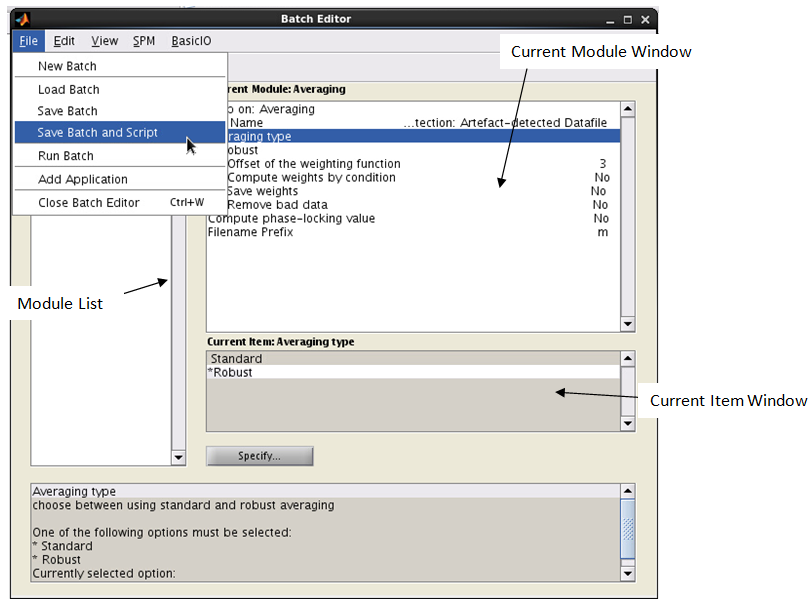
\includegraphics[width=120mm]{multi/figures/figure1}
\caption{\em Screenshot of the Batch Editor. The Module List, Current Module Window and Current Item Windows are identified. The cursor highlights how to save the pipeline as a batch and script. \label{multi:fig:1}}
\end{center}
\end{figure}

\section{Preprocessing M/EEG data}

We will start by creating pipelines (using SPM's batch interface) for preprocessing the M/EEG data for a single subject, and then scripting these pipelines to repeat over multiple subjects. For no particular reason, we will start with Subject 15.

\subsection{Convert (and epoch)}

The first step is to convert raw M/EEG data from its native format (which depends on the acquisition system) to the format used by SPM.  In the present example, the raw data are continuous. They can be converted to continuous SPM data, but to save disk space and time, we can ``cut out'' time windows (epochs) around the trials during the conversion step, so that the resulting SPM file contains epoched data.

In the batch editor, select SPM on the top toolbar, and from the dropdown menu select M/EEG. At the top of the new dropdown menu, select ``Conversion''. Once selected, the Module List on the left of the batch editor window will now list ``Conversion'' as the first (and only) step. Within the main, Current Module window will be listed several variables. The first variable listed is ``File Name''. On the right hand of this pane, you will see ``\(<\)-X'', this indicates that you need to update this field. To do so, click on ``File Name'', this will then open up your current working directory. For this example we will be using the M/EEG data from subject number 15 (in the \texttt{Sub15} directory). Select the file named \texttt{run\_01\_sss.fif} and press ``Done''.

Many variables in the Current Module window have default values, but we need to change some of them. For example, we want to epoch during conversion, so highligh the ``reading mode'' and change from ``continuous'' to ``epoched''. To epoch, we need to define the start and end of each trial. This information normally comes from a trigger channel containing pulses that encode the onset and type of trial. You can ask SPM to read this channel and select the relevant trial codes by hand. However, here we will use ``trial definition'' files that have been created in advance (given the complexity of the trigger codes in this dataset; contact authors for more information on trial definitions). So select ``Trial definition file'' under the ``epoched'' option, click on ``Specify'' and select the file \texttt{run\_01\_trldef.mat}. (The contents of this file conform to the FieldTrip format, with one row per trial, each with three columns, which represent the sample numbers from the start of the continuous recording for 1) onset of the epoch, 2) offset of the epoch and 3) pre-stimulus baseline period.) Each trial runs from -500ms to +1200ms relative to the stimulus onset. (In fact, we only really care about the period -100ms to +800ms in the analysis below, and will later ``crop'' the trials to this period, but we first need the extra 400ms at the start and end to provide ``padding'' to avoid ``end-effects'' in the wavelet analysis done later.)

Another change to the defaults is that we do not want to convert all channels in the original file (since many are extraneous), so will select a subset by their type. We first need to delete the default option to convert all channels. To do this, click ``channel selection'', and  scroll down until you can select the ``Delete All(1)'' option. Then click the ``channel selection'' again, but this time choose the option ``New: Select channels by type''. This will add ``Select channels by type'' to the Current Module, and you will see ``\(<\)-X'' on the right hand side of this, indicating the need for user input. Click the ``\(<\)-X'' and then select ``EEG'' from the ``Current Item'' section. Repeat this process to additionally include the ``MEGMAG'' and ``MEGPLANAR'' channels.

The remaining options for conversion can be left with their default values (which includes the output filename, which defaults to the input filename, simply prepended with \texttt{spmeeg\_}). Once all variables are specified, the ``play'' button on the top toolbar will turn green and the batch could be run. However, for this example, we will continue to use the current batch editor window, so do not press the ``play'' button yet.

\subsection{Prepare}

The next step in the current pipeline is to update some other properties of the data using the ``Prepare'' module. This is a general-purpose ``housekeeping'' module that includes options like re-defining channel names, types, locations, etc. as specific to the particular laboratory set-up. In our case, some of channels currently labelled EEG were in fact used to record EOG.

Select ``Prepare'', from the preprocessing menu. Highlight ``Prepare'' in the Module list, this will open up the variables in the current module window. Again we need to complete those variables indicated by the ``\(<\)-X''. If we had already run the previous conversion stage, we could select the new \texttt{spmeeg\_run\_01\_sss.mat} file produced by that stage as the input for this stage. Here however, we will create a pipeline in which all stages are run in one go, in which case we need to tell SPM that the output of the conversion step, even though not yet created, will be the input of this preparation step. You can do this by selecting the ``Dependency'' button located further down the window. This will open up a new window, listing all the processing steps up to this point. So far this is just one, the conversion step. Highlight this step and select ``OK''.

The next variable to define is the ``task(s)''. Clicking this variable will display a variety of options in the ``current item'' box. Within this, select ``New: Set channel type'', then return to the current module window. In here, highlight ``Channel selection'', which displays further variables within the current item window. Select ``New: Custom channel''. Now return to the current module box and select the variable with an ``\(<\)-X''. This should be ``Custom channel''. Selecting this and clicking on ``Specify'' will open up a small text window. Within this, type \texttt{EEG061}. Create a new Custom channel and type \texttt{EEG062}; then select ``new channel type'' and highlight ``EOG''. This is because channels EEG061 and EEG062 in fact represented bipolar horizontal (HEOG) and vertical (VEOG) electroculagrams respectively, which can be used to detect ocular artifacts.

This process then needs to be repeated for two other new channel types. First create a new channel type like above, label it \texttt{EEG063} and set its channel type as ``ECG''. This channel represents the electrocardiogram, which can be used to detect cardiac artifacts. Second, create another new channel labelled \texttt{EEG064} and set its channel type as ``other'' (this is just a free-floating electrode, and does not contain data of interest).

One more job we need to do is specify ``bad'' channels. These only exist for the EEG (MEG bad channels are assumed to be corrected by the prior MaxFiltering step). Bad EEG channels were identified by hand by an experienced EEG operator and saved in a file called \texttt{bad\_channels.mat} in each subject's directory. It is important to note that there are many other ways that bad channels can be defined automatically by SPM, using the ``artefact'' module for example, but the various options for this are not explored in this chapter. To specify bad channels, add a second Prepare module, select the ``New: Set/unset bad channels'', then under ``Channel selection'', replace the default ``All'' with the option ``New: Channel file'', and then select the \texttt{bad\_channels.mat} file in this subject's directory (note it is important that you delete the ``All (1)'' option first). In fact, this subject does not have any bad channels, so this step could be ignored if you only want to analyse this subject. But if you want to use the preprocessing script that we will use below for the remaining 15 subjects, you need to set-up this stage now (i.e, the \texttt{bad\_channels.mat} files for the other subjects are not empty).

This will complete the preparation stage, as indicated by the ``play'' button turning green. (Note that you can also use this ``Prepare'' option interactively, in order, for example, to create and save a bad channel selection file).

\subsection{Downsample}

The data were sampled at 1000Hz, but for the analyses below, we rarely care about frequencies above 100Hz. So to save processing time and disk space (by a factor of 5) we can therefore downsample the data to 200Hz (which includes a lowpass filtering to avoid aliasing). Select ``downsampling'' from the module list ``SPM -- M/EEG -- Preprocessing'', click on ``File Name'', select ``Dependency'' and in the pop-up window, select the prepared datafile at the bottom of the list. Next, set the downsampling rate by clicking the ``New sampling rate'' variable within the current module box. Type \texttt{200} into the pop-up window that appears and use ``OK'' to set this value. The output file of this stage will be prepended with a \texttt{d}. 

\subsection{Baseline Correction}

The next step in this preprocessing pipeline is to baseline correct the data by subtracting from each channel the mean from -100ms to 0ms relative to the stimulus onset. Select ``Baseline Correct'' from under the ``SPM -- M/EEG -- Preprocessing'' menu. Select the input file name as being dependent on the output of the downsampling by selecting the ``Dependency''. To define the baseline, highlight the ``Baseline'' button in the current module window and click on the ``Specify'' button. The baseline needs to be entered as a 1-by-2 array. Enter \texttt{[-100 0]} (units are milliseconds). The prefix of this file name will be \texttt{b}. Note, that to be on the safe side it might be a good idea to perform baseline correction before downsampling. The reason is that in the general case there might be large DC offsets in the data leading to prolonged ringing that even padding will not protect against. For our data, however, the order shown here works equally well.

\subsection{Deleting intermediate steps (optional)}

The four steps (modules) described above create a preprocessing pipeline for the data. If this pipeline is run straight away, there will be four different output files. If you are short of diskspace, you might want to delete some of the intermediate files. To do this, select ``SPM'' from the top toolbar of the batch editor window and choose ``M/EEG -- Other -- Delete'' several times. Then you will need to specify the File Names to delete. Highlight each ``Delete'' module and set the File Name as the output of the Prepare step using the ``Dependency'' button to delete any output from the conversion/prepare step onward. In fact, all processing steps up until the most recent step (Baseline-correction) can be deleted. To do this, right click on ``Delete'' in the Module List and select ``Replicate Module'', but change the dependency to the downsampled file. 

\paragraph{Creating a script for combining pipelines within a subject.}

Once you have created a linear pipeline, you might want to repeat it on multiple sessions (runs) within a subject, or even across multiple subjects. In the present case, there were 6 independent MEG runs (separated only by a short period to give the subjects a rest), which can all be processed identically. One option would be to save the batch file, manually alter the ``File Name'' that is initially loaded into the batch editor, and repeat this process separately for each run. A more powerful approach is to create a script. To do this, select ``File'' from the Batch Editor window, and select ``Save Batch and Script''. This will produce two files: a batch file (same as that created when you save a batch) but also a \matlab\ script that calls that batch file. So if you call the batch file \texttt{batch\_preproc\_meeg\_convert}, you will get a batch file called \texttt{batch\_preproc\_meeg\_convert\_job.m} and a script file called \texttt{batch\_preproc\_meeg\_convert.m}.
 
The script file \texttt{batch\_preproc\_meeg\_convert.m} will automatically be loaded into the \matlab\ editor window, and should appear something like this:


\begin{lstlisting}[style=Matlab-editor,basicstyle=\mlttfamily\footnotesize]
% List of open inputs
% Conversion: File Name - cfg_files
% Conversion: Trial File - cfg_files
% Prepare: Channel file - cfg_files
nrun = X; % enter the number of runs here
jobfile = {'batch_preproc_meeg_convert_job.m'};
jobs = repmat(jobfile, 1, nrun);
inputs = cell(3, nrun);
for crun = 1:nrun
    inputs{1, crun} = MATLAB_CODE_TO_FILL_INPUT; % Conversion: File Name - cfg_files
    inputs{2, crun} = MATLAB_CODE_TO_FILL_INPUT; % Conversion: Trial File - cfg_files
    inputs{3, crun} = MATLAB_CODE_TO_FILL_INPUT; % Prepare: Channel file - cfg_files
end
spm('defaults', 'EEG');
spm_jobman('run', jobs, inputs{:}); 
\end{lstlisting}

At the top of this script is listed the variable \verb|nrun = X|: replace \verb|X| with \verb|6| for the six runs you wish to convert. You also need to complete the missing \matlab\ code needed for each run: here, 1) the raw input file to convert, 2) the trial definition file for that run, and 3) the channel file containing the bad channels (which is actually the same for each run, but differs across subjects, which will matter later when we extend the script to loop over subjects). In order to automate selection of these files, you need to know some basic \matlab\ . For example, because the files are named systematically by run, we can complete the relevant lines of the script with:

\begin{lstlisting}[style=Matlab-editor,basicstyle=\mlttfamily\footnotesize]
     inputs{1, crun} = cellstr(fullfile(rawpth,'Sub15','MEEG',sprintf('run_%02d_sss.fif',crun)));
     inputs{2, crun} = cellstr(fullfile(rawpth,'Sub15','MEEG','Trials',sprintf('run_%02d_trldef.mat',crun)));
     inputs{3, crun} = cellstr(fullfile(rawpth,'Sub15','MEEG','bad_channels.mat'));
\end{lstlisting}

where \verb|rawpth| refers to your base directory, \verb|Sub15| is the subject directory that contains \texttt{MEG} and \texttt{Trials} sub-directories (assuming you mirrored the directory structure from the FTP site) and \texttt{\%02d} refers to the run number, expressed as two digits.

The other file -- the batch or ``job'' file -- can be reloaded into the batch editor at any time. It can also be viewed in the \matlab\ editor. If you type \texttt{edit batch\_preproc\_meeg\_convert\_job.m}, you will see your selections from the earlier GUI steps. But we need to change those selections that depend on the run number (so they can be passed from the script instead). To make the batch file accept variables from the script file, we need change three of the specifications to \texttt{'<UNDEFINED>'} instead. So edit the following lines so they read:

\begin{lstlisting}[style=Matlab-editor,basicstyle=\mlttfamily\footnotesize]
     matlabbatch{1}.spm.meeg.convert.dataset = '<UNDEFINED>';
     matlabbatch{1}.spm.meeg.convert.mode.epoched.trlfile = '<UNDEFINED>';
     ...
     matlabbatch{2}.spm.meeg.preproc.prepare.task{4}.setbadchan.channels{1}.chanfile = '<UNDEFINED>';
\end{lstlisting}

Then save these edits (overwriting the previous batch file). If you're unsure, the batch file should look like the \texttt{batch\_preproc\_meeg\_convert\_job.m} file in the \texttt{SPM12batch} part of the \texttt{SPMscripts} directory on the FTP site. 

This completes the first part of the preprocessing pipeline. You can then run this script by selecting the green play button on the upper toolbar of the script \matlab\ Editor window. The results will be 6 files labelled \texttt{bdspmeeg\_run\_\%02d\_sss.mat}, where \texttt{\%02d} refers to the run number \verb|1-6|. If you want to view any of these output files, press ``Display'' on the main SPM menu pane, select ``M/EEG'', then select one of these files. You will be able to review the preprocessing steps as a pipeline from the ``History'' section of the ``Info'' tab, and can view single trials by selecting one of the EEG, MEG (magnetometer) or MPLANAR (gradiometer) tabs (see other chapters for how to use the buttons in the M/EEG Review window).

\subsection{Merging (concatenating runs)}

To analyse the data as one file, the six runs need to be merged. To do this, select ``Merging'' from ``SPM -- M/EEG -- Preprocessing -- Merging'', select ``File Names'', ``specify'', and select the 6 file names \texttt{bdspmeeg\_run\_\%02d\_sss.mat}. If you were to run this stage now, the output file would match the first input file, but be prepended with a \texttt{c}, i.e, \texttt{cbdspmeeg\_run\_01\_sss.mat}. However, we will wait to add some more modules before running, as below. At this stage, you could also add delete modules to delete all the previous individual run files (since the concatenated file will contain all trials from all runs, i.e, contain the same data).

\subsection{Prepare (a montage for re-referencing the EEG)}

Below, we want to re-reference the EEG data to the average across channels (as is sometimes conventional for ERP analyses; note the MEG data have no reference). We can do this with the ``montage'' module below, which is a general purpose module for creating new channel data from linear combinations of existing channel data. However, we first need to create a montage file, which includes a matrix that, when multiplied by the existing data, creates the new channel data. There is another sub-function (task) of the ``Prepare'' module that does this, so add another ``Prepare'' module, select the dependency on the previous merged file as the ``FileName'', but for the ``task'', select ``Create average reference montage'' and enter \texttt{avref\_montage.mat} as the output filename. (If you want to look at this montage, you can run this module, \texttt{load avref\_montage.mat} into \matlab\ and look at the \texttt{montage.tra} matrix, where you can see that each new EEG channel is equal to the old EEG channel minus the average of all other channels.)  Note that this montage will differ across subjects because different subjects had different EEG channels marked as bad (from steps above), and bad channels need to be excluded when estimating the average EEG signal across channels.

At this point, we can also do one more bit of house-keeping within the same ``Prepare'' module, which is simply to re-order the condition labels. This only matters for the final stage of ``Contrasting conditions'' below, where the contrast weights assume a certain order of the conditions. The current order of conditions is based purely on the order they appear in the raw data (e.g, if the first few trials of the first run were: Scrambled, Unfamiliar, Unfamiliar, Scrambled, Famous..., then the condition labels will be ordered Scrambled-Unfamiliar-Famous), and this may vary across subjects. To set the condition order to be invariant across subjects, add a new task by selecting the ``Sort conditions'' task, then ``Specify conditions lists'' add three ``New: Condition labels'', and name them ``Famous'', ``Unfamiliar'' and ``Scrambled'' (in that order). Note that this operation does not physically reorder the trials at this stage, but just defines the order that will be used where required at later steps.

\subsection{Montage}

Now we have the montage file, we can apply it, in order to re-reference the EEG data to the average. Select ``Montage'' from the ``Preprocessing'' menu, and specify the ``File Name'' as being dependent on the output of the ``Merging'' module above. For the ``Montage file name'', choose a different dependency, namely the output of the ``Prepare'' module above. Next, highlight ``keep other channels'' and select ``yes'' in the ``Current Item'' box, in order to keep all the MEG channels (which are unchanged). All other default values can remain the same. The output file will be prepended with \texttt{M}.

As with the previous pipeline, if you are short of diskspace (particularly if you later run all 16 subjects), the outputs produced from the intermediate stages can be deleted using the ``SPM -- M/EEG -- Other -- Delete'' function (see earlier). However, refrain from deleting the montaged data, as these will be used later in the Section on Time-Frequency analysis.

\paragraph{Save batch and review.}

This completes the second part of the preprocessing pipeline. At this point, you can run the batch. Alternatively, you can save and script, and run the batch from a script. The resulting script can also be combined with the previous script created (e.g., in the \texttt{SPMscripts} FTP directory, scripts for all the stages are appended into a single master script called \texttt{master\_script.m}, which loops over each subject too). Remember that, if you want to pass variables from a script to a batch, you need to first ensure the relevant fields in the batch file are set to \texttt{'<UNDEFINED>'} (see for example the \texttt{batch\_preproc\_meeg\_merge\_job.m} file in the \texttt{SPM12batch} FTP directory).
 
To view the output, press ``Display'' on the main SPM menu pane, select ``M/EEG'', then select \texttt{Mcbdspmeeg\_run\_01\_sss.mat}. Again, you will be able to review the preprocessing steps from the ``History'' section of the ``Info'' tab. 

\section{Evoked analysis}

At this point, the preprocessing forks into two strands: one for trial-averaged amplitude analysis and one for time-frequency analysis. The first of these corresponds to a typical evoked response (ER) analysis, where we simply average across trials in each condition (note this will attenuate any non-phase locked, i.e. induced responses; to detect these, we will later perform time-frequency analysis before averaging). Before averaging though, we will crop the 400ms buffer around each trial (which is only necessary for the time-frequency analysis).

\subsection{Crop}

To crop the data, select the crop option from ``SPM -- M/EEG -- Preprocessing -- Crop''. Select the datafile called \texttt{Mcbdespmeeg\_run\_01\_sss.mat} produced from the final EEG re-referencing (``Montage'') step above.  A 100ms pre-stimulus baseline period is normally sufficient, and we do not care about responses after 800ms for this particular analysis, so we can cut off 400ms at the start and end of each trial to produce an epoch from -100ms to +800ms. To do this, select ``Time Window'' from the ``Current Module'' window, then the ``Specify'' button. Within the pop up window, enter \texttt{[-100 800]} as a 1-by-2 array. The channel selection will be ``all''. This file output will be prepended with a \texttt{p}.

\subsection{Artefact detection}

There are many ways to define artifacts (including special toolboxes; see other SPM manual chapters). Here we focus on just one simple means of detecting blinks by thresholding the EOG channels. Select ``Artefact detection'' from the ``SPM -- M/EEG -- Preprocessing'' menu. For the input file, select a dependency on the output of the previous step (``Crop''). Next, select ``New: Method'' from the box titled ``Current Item: How to look for artefacts''. Back in the ``Current Module'' window, highlight ``Channel selection'' to list more options, choose ``Select channels by type'' and select ``EOG''. Then do not forget to also delete the default ``All'' option! Then press the ``\(<\)-X'' to select ``threshold channels'', click the ``Specify'' button and set this to \texttt{200} (in units of microvolts). The result of this thresholding will be to mark a number of trials as ``bad'' (these can be reviewed after the pipeline is run if you like). Bad trials are not deleted from the data, but marked so they will be excluded from averaging below. The output file will be prepended with the letter ``a''. 

\subsection{Combine Planar Gradiometers}

The next step is only necessary for scalp-time statistics on planar gradiometers. For scalp-time images, one value is needed for each sensor location. Neuromag's planar gradiometers measure two orthogonal directions of the magnetic gradient at each location, so these need to be combined into one value for a scalar (rather than vector) topographic representation. The simplest way to do this is to take the Root Mean Square (RMS) of the two gradiometers at each location (i.e. estimate the 2D vector length). In SPM, this will create a new sensor type called MCOMB. Note that this step is NOT necessary for source reconstruction (where, the forward model captures both gradiometers). Note also that the RMS is a nonlinear operation, which means that zero-mean additive noise will no longer cancel by averaging across trials, in turn meaning that it is difficult to compare conditions that differ in the number of trials. To take the RMS, select ``Combine Planar'' from the ``SPM -- M/EEG -- Preprocessing'' menu, highlight ``File Name'', select the ``dependency'' button, and choose the Artefact-corrected file above. Leave the ``copying mode'' as default -- ``Replace planar''.  The produced file will be prepended with \texttt{P}.

\subsection{Trial averaging}

To average the data across trials, select ``SPM -- M/EEG -- Average -- Averaging'', and define the input as dependent on the output of the planar combination module. Keep the remaining options as the default values. (If you like, you could change the type of averaging from ``standard'' to ``Robust''. Robust averaging is a more sophisticated version of normal averaging, where each timepoint in each trial is weighted according to how different it is from the median across trials. This can be a nice feature of SPM, which makes averaging more robust to atypical trials, though in fact it does not make much difference for the present data, particularly given the large numbers of trials, and we do not choose it here simply because it takes much longer than conventional averaging.) Once completed, this file will have a prefix of \texttt{m}.

\subsection{Contrasting conditions}

We can also take contrasts of our trial-averaged data, e.g., to create a differential ER between faces and scrambled faces. This is sometimes helpful to see condition effects, and plot their topography. These contrasts are just linear combinations of the original conditions, and so correspond to vectors with 3 elements (for the 3 conditions here). Select ``SPM -- M/EEG -- Average -- Contrast over epochs'', and select the output of ``Averaging'' above as in the dependent input. You can then select ``New Contrast'' and enter as many contrasts as you like. The resulting output file is prepended with \texttt{w}.

For example, to create an ER that is the difference between faces (averaged across Famous and Unfamiliar) and scrambled faces, enter the vector \verb|[0.5 0.5 -1]| (assuming conditions are ordered Famous-Unfamiliar-Scrambled; see comment earlier in ``Prepare'' module), and give it a name. Or to create the differential ER between Famous and Unfamiliar faces, enter the vector \verb|[1 -1 0]|. Sometimes it is worth repeating the conditions from the previous averaging step by entering, in this case, three contrasts: \verb|[1 0 0]|, \verb|[0 1 0]| and \verb|[0 0 1]|, for Famous, Unfamiliar and Scrambled conditions respectively. These will be exactly the same as in the averaged file above, but now we can examine them, as well as the differential responses, within the same file (i.e. same graphics window when we review that file), and so can also delete the previous \texttt{m} file.

\paragraph{Save batch and review.}

At this point, you can save batch and script again. The resulting batch file should look like the \texttt{batch\_preproc\_meeg\_erp\_job.m} file in the \texttt{SPM12batch} part of the \texttt{SPMscripts} FTP directory. The script file can be run (and possibly combined with the previous script created).

We will start by looking at the trial-averaged ERs to each of the three conditions. Select the ``Display'' button on the SPM Menu and select the file \texttt{wmPapMcbdspmeeg\_run\_01\_sss.mat}. Then select, for example, the ``EEG'' tab, and you will see each channel as a row (``strip'', or ``standard view'') for the mean ER for Famous faces. If you press ``scalp'' instead, the channels will be flat-projected based on their scalp position (nose upwards). You can now display multiple conditions at once by holding the shift-key and selecting Trials 2 and 3 (Unfamiliar and Scrambled) as well (as in Figure~\ref{multi:fig:2}, after zooming the y-axis slightly). If you press the expand y-axis button (top left) a few times to up-scale the data, you should see something like in Figure~\ref{multi:fig:2}. You can see the biggest evoked potentials (relative to average over channels) at the back of the head.

\begin{figure}
\begin{center}
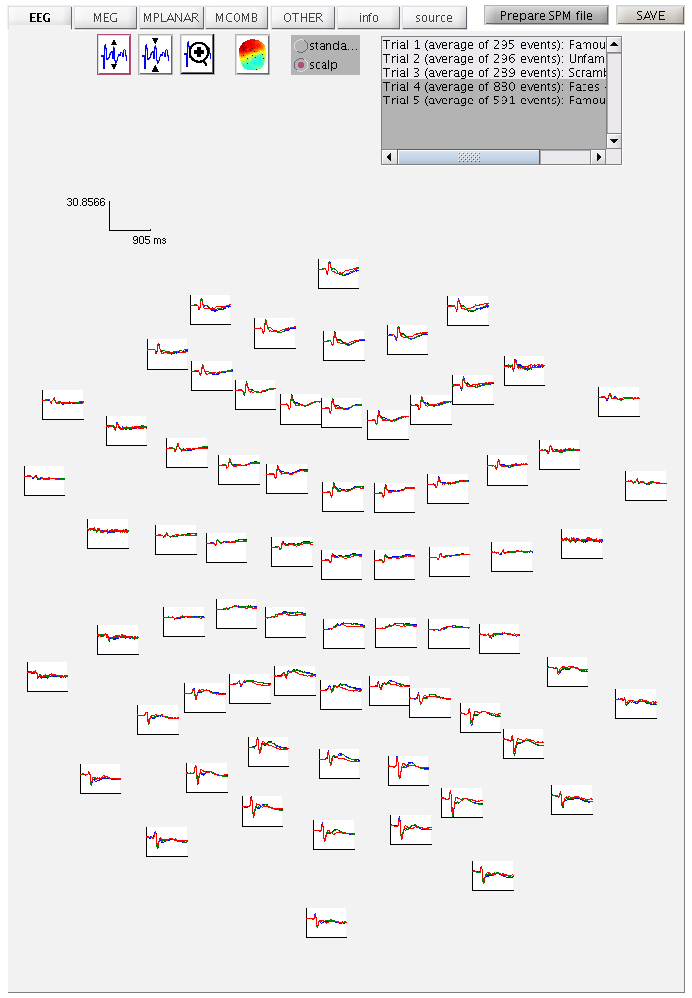
\includegraphics[width=100mm]{multi/figures/figure2}
\caption{\em Trial-averaged ERPs for each condition over all EEG channel positions on the scalp. \label{multi:fig:2}}
\end{center}
\end{figure}

If you press the magnifying glass icon, then with the cross-hairs select Channel 70 (in bottom right quadrant of display), you will get a new figure like in Figure~\ref{multi:fig:3} that shows the ERPs for that channel in more detail (and which can be adjusted using the usual \matlab\ figure controls). You can see that faces (blue and green lines) show a more negative deflection around 170ms than do scrambled faces (red line), the so-called ``N170'' component believed to index the earliest stage of face processing.

\begin{figure}
\begin{center}
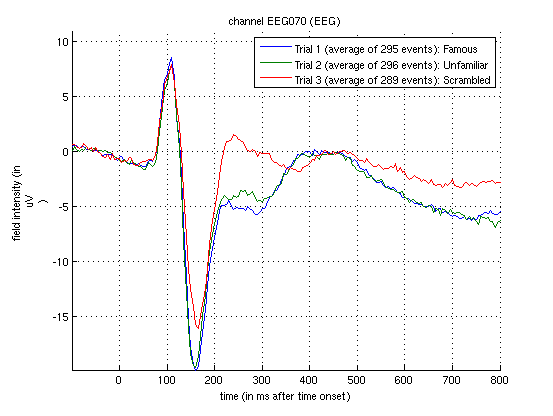
\includegraphics[width=100mm]{multi/figures/figure3}
\caption{\em Trial-averaged ERPs for each condition from EEG channel 70 (right posterior). \label{multi:fig:3}}
\end{center}
\end{figure}

To see the topography of this differential N170 component, select instead the fourth trial (contrast) labelled ``Faces -- Scrambled''. Then press the coloured topography icon, and you will get a new figure with the distribution over the scalp of the face-scrambled difference. If you shift the time-slider on the bottom of that window to the leftmost position, and then repeatedly click on the right arrow, you will see the evolution of the face effect, with no consistent difference during the prestimulus period, or until about 155ms, at which point a clear dipolar field pattern should emerge (Figure~\ref{multi:fig:4}). 

\begin{figure}
\begin{center}
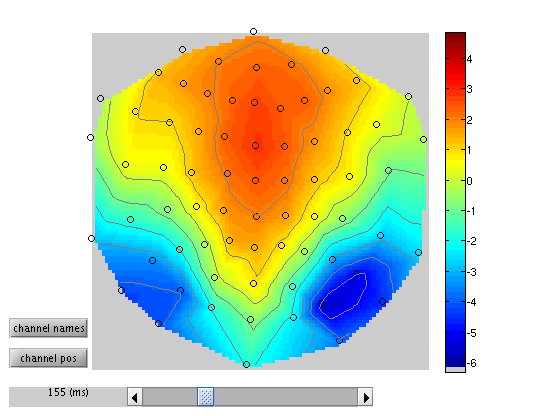
\includegraphics[width=100mm]{multi/figures/figure4}
\caption{\em Topography of differential ERP for faces (famous and unfamiliar) vs scrambled at 155ms. \label{multi:fig:4}}
\end{center}
\end{figure}

You can of course explore the other sensor-types (magnetometers, MEG) and combined gradiometers (MCOMB), which will show an analogous ``M170''. You can also examine the EOG and ECG channels, which appear under the ``OTHER'' tab. (Note that the VEOG channel contains a hint of an evoked response: this is not due to eye-movements, but due to the fact that bipolar channels still pick up a bit of brain activity too. The important thing is that there is no obvious EOG artefact associated with the difference between conditions, such as differential blinks.)

But how do we know whether this small difference in amplitude around 150-200ms is reliable, given the noise from trial to trial? And by looking at all the channels and timepoints, in order to identify this difference, we have implicitly performed multiple comparisons across space and time: so how do we correct for these multiple comparisons (assuming we had no idea in advance where or when this face-related response would occur)? We can answer these questions by using random field theory across with scalp-time statistical parametric maps. But first, we have to convert these sensor-by-time data into 3D images of 2D-location-by-time.

\subsection{Time-Sensor images}

To create 3D scalp-time images for each trial, the 2D representation of the scalp is created by projecting the sensor locations onto a plane, and then interpolating linearly between them onto a 32\(\times\)32 pixel grid. This grid is then tiled across each timepoint. To do this, you need to select the ``SPM -- M/EEG -- Images -- Convert2Images'' option in the batch editor. For the input file, select the \texttt{PapMcbdspmeeg\_run\_01\_sss.mat} file that contains every cropped trial (i.e, before averaging), but with bad trials marked (owing to excessive EOG signals; see earlier). Next select ``Mode'', and select ``scalp x time''. Then, select ``conditions'', select ``Specify'' and enter the condition label ``Famous''. Then repeat for the condition labels ``Unfamiliar'' and ``Scrambled''. 

To select the channels that will create your image, highlight the ``Channel selection'', and then select ``New: Select channels by type'' and select ``EEG''. The final step is to name the Directory prefix \texttt{eeg\_img\_st} this can be done by highlighting ``directory prefix'', selecting ``Specify'', and the prefix can then be entered.

This process can be repeated for the MEGMAG channels, and the MEGCOMB channels (although we will focus only on the EEG here). If so, the easiest way to do this is to right-click ``Convert2Images'' in the Module List, and select ``replicate module''. You will have to do this twice, and then update the channels selected, and the directory prefix to \texttt{mag\_img\_mat} and \texttt{grm\_img\_mat} to indicate the magnetometers (MEGMAG) and the gradiometers (MEGCOMB) respectively. 

\paragraph{Save batch and review.}

At this point, you can save batch and script again. The resulting batch file should look like the \texttt{batch\_preproc\_meeg\_erp\_images\_job.m} file in the \texttt{SPM12batch} FTP directory. Once you have run this script, a new directory will be created for each channel-type, which is based on the input file and prefix specified above (e.g., \texttt{eeg\_\-img\_\-st\_\-PapMcbdspmeeg\_\-run\_01\_sss} for the EEG data). Within that directory will be three 4D NIfTI files, one per condition. It is very important to note that these 4D files contain multiple ``frames'' (i.e. 3D scalp-time images), one per trial (i.e. 296 in the case of unfamiliar faces). To view one of these, press ``Display -- Images'' in the SPM Menu window, and select, say, the \texttt{condition\_Unfamiliar.nii} file. But note that by default you will only see the first scalp-time image in each file (because the default setting of ``Frames'' within the Select Image window is \texttt{1}). To be able to select from all frames, change the ``Frames'' value from \texttt{1} to \texttt{Inf} (infinite), and now you will see all 296 frames (trials) that contained Unfamiliar faces. If you select, say, number 296, you should see an image like in Figure~\ref{multi:fig:5} (this was created after selecting ``Edit -- Colormap'' from the top toolbar, then ``Tools -- Standard Colormap -- Jet'', and entering \verb|[0 0 165]| as the coordinates in order to select 165ms post-stimulus). You can scroll will the cross-hair to see the changes in topography over time.

\begin{figure}
\begin{center}
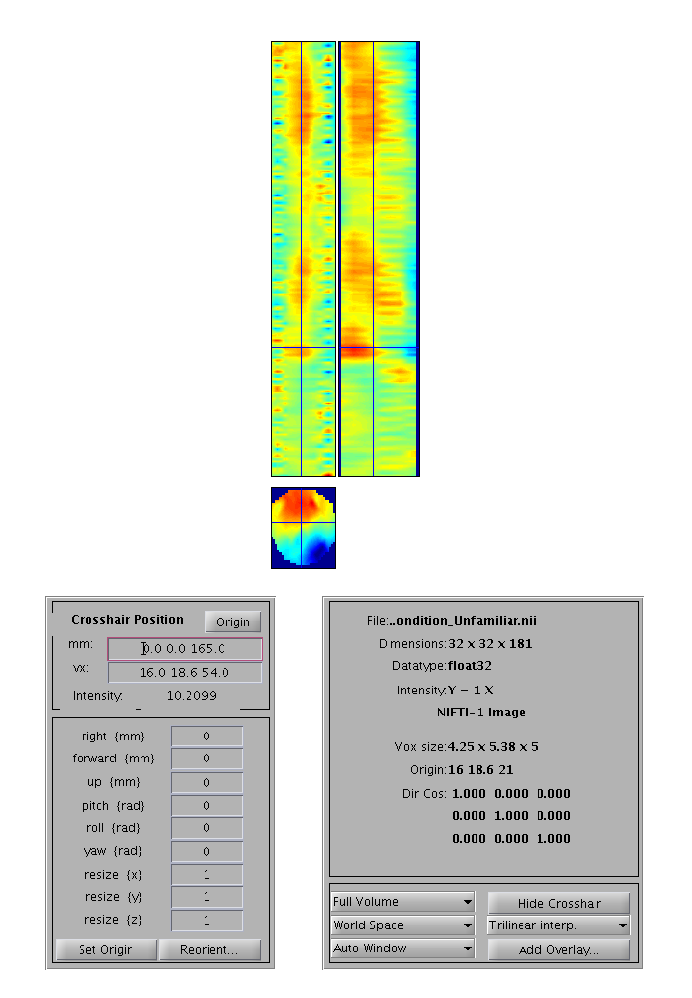
\includegraphics[width=150mm]{multi/figures/figure5}
\caption{\em 3D Scalp-Time image for 296th trial in the Unfamiliar condition. \label{multi:fig:5}}
\end{center}
\end{figure}


Note that Random Field Theory, used to correct the statistics below, assumes a certain minimum smoothness of the data (at least three times the voxel size). The present data meet this requirement, but in other cases, one could add an additional step of Gaussian smoothing of the images to ensure this smoothness criterion is met.  

\section{Scalp-Time Statistics across trials within one subject}

Now we have one image per trial (per condition), we can enter these into a GLM using SPM's statistical machinery (as if they were fMRI or PET images). If we ignore temporal autocorrelation across trials, we can assume that each trial is an independent observation, so our GLM corresponds to a one-way, non-repeated-measures ANOVA with 3 levels (conditions).

\subsection{Model Specification}

To create this model, open a new batch, select ``Factorial design specification'' under ``Stats'' on the SPM toolbar at the top of the batch editor window. The first thing is to specify the output directory where the SPM stats files will be saved. So first create such a directory within the subject's sub-directory, calling it for example \texttt{STStats}, and then create a sub-directory \texttt{eeg} within \texttt{STStats} (and potentially two more called \texttt{mag} and \texttt{grm} if you want to examine other sensor-types too). Then go back to the batch editor and select this new \texttt{eeg} directory.

Highlight ``Design'' and from the current item window, select ``One-way ANOVA''. Highlight ``Cell'',  select ``New: Cell'' and repeat until there are three cells. Select the option ``Scan'' beneath each ``Cell'' heading (identified by the presence of a ``\(<\)-X''). Select ``Specify'', and in the file selector window, remember to change the ``Frames'' value from \texttt{1} to \texttt{Inf} as previously to see all the trials. Select all of the image files for one condition (by using the right-click ``select all'' option).  It is vital that the files are selected in the order in which the conditions will later appear within the Contrast Manager module (i.e., Famous, Unfamiliar, Scrambled). Next highlight ``Independence'' and select ``Yes'', but set the variance to ``Unequal''. Keep all the remaining defaults (see other SPM chapters for more information about these options).

Finally, to make the GLM a bit more interesting, we will add 3 extra regressors that model the effect of time within each condition (e.g. to model practice or fatigue effects). (This step is optional if you'd rather omit.) Press ``New: Covariate'' under the ``Covariates'' menu, and for the ``Name'', enter ``Order Famous''. Keep the default ``None'' to interactions, and ``Overall mean'' for ``centering''. We now just need to enter a vector of values for every trial in the experiment. These trials are ordered Famous, Unfamiliar and Scrambled, since this is how we selected them above. So to model linear effects of time within Famous trials, we need a vector that goes from \texttt{1:295} (since there are 295 Famous trials). However, we also need to mean-correct this, so we can enter \texttt{detrend([1:295],0)} as the first part of the vector (covariate) required. We then need to add zeros for the remaining Unfamiliar and Scrambled trials, of which there are 296+289=585 in total. So the complete vector we need to enter (for the Famous condition) is \texttt{[detrend([1:295],0) zeros(1,585)]}. We then need to repeat this time covariate for the remaining two conditions. So press ``New: Covariate'' again, but this time enter ``Order Unfamiliar'' as the name, and \texttt{[zeros(1,295) detrend([1:296],0) zeros(1,289)]} as the vector. Finally, press ``New: Covariate'', but this time enter ``Order Scrambled'' as the name, and \texttt{[zeros(1,591) detrend([1:289],0)]} as the vector.

This now completes the GLM specification, but before running it, we will add two more modules.

\subsection{Model Estimation}

The next step within this pipeline is to estimate the above model. Add a module for ``Model Estimation'' from the ``Stats'' option on the SPM toolbar and define the file name as being dependent on the results of the factorial design specification output. For ``write residuals'', keep ``no''. Select classical statistics.

\subsection{Setting up contrasts}

The final step in the statistics pipeline is create some planned comparisons of conditions by adding a ``Contrast Manager'' module from the ``Stats'' bar. Define the file name as dependent on the model estimation. The first contrast will be a generic one that tests whether significant variance is captured by the 6 regressors (3 for the main effect of each condition, and 3 for the effects of time within each condition). This corresponds to an F-contrast based on a 6x6 identity matrix. Highlight contrast sessions and select a new F-contrast session. Name this contrast ``All Effects''. Then define the weights matrix by typing in \texttt{eye(6)} (which is \matlab\ for a 6\(\times\)6 identity matrix). (Since there is only one ``session'' in this GLM,  select ``Don't replicate'' from the  ``replicate over sessions'' question.) We will use this contrast later to plot the parameter estimates for these 6 regressors.

More interestingly perhaps, we can also define a contrast that compares faces against scrambled faces (e.g. to test whether the N170 seen in the average over trials in right posterior EEG channels in Figure~\ref{multi:fig:3} is reliable given the variability from trial to trial, and to also discover where else in space or time there might be reliable differences between faces and scrambled faces). So make another F-contrast, name this one ``Faces (Fam+ Unf) \(<>\) Scrambled'', and type in the weights \texttt{[0.5 0.5 -1 0 0 0]} (which contrasts the main effect of faces vs scrambled faces, ignoring any time effects (though SPM will complete the final zeros if you omit). Note that we use an F-test because we don't have strong interest in the polarity of the face-scrambled difference (whose distribution over the scalp depends on the EEG referencing). But if we did want to look at just positive and negative differences, you could enter two T-contrasts instead, with opposite signs on their weights.

\paragraph{Save batch and review}

Once you have added all the contrasts you want, you can save this batch file (it should look like the \texttt{batch\_stats\_ANOVA\_job.m} file in the \texttt{SPM12batch} FTP directory). This only runs a GLM for one sensor-type (we cannot combine the sensors until we get to source space later), so you can write a script around this batch that calls it three times, once per sensor-type (i.e, for magnetometers and gradiometer RMS too), just changing the output directory and input files (see \texttt{master\_script.m} on the \texttt{SPM12batch} FTP directory).

The results of this output can be viewed by selecting ``Results'' from the SPM Menu window. Select the \texttt{SPM.mat} file in the \texttt{STStats/eeg} directory, and from the new ``Contrast Manager'' window, select the pre-specified contrast ``Faces (Fam+Unf) \(<>\) Scrambled''.  Within the Interactive window which will appear on the left hand side, select the following:  Apply Masking: None, P value adjustment to control: FWE, keep the threshold at 0.05, extent threshold \{voxels\}: 0; Data Type: Scalp-Time. The Graphics window should then show what is in Figure~\ref{multi:fig:6}.

\begin{figure}
\begin{center}
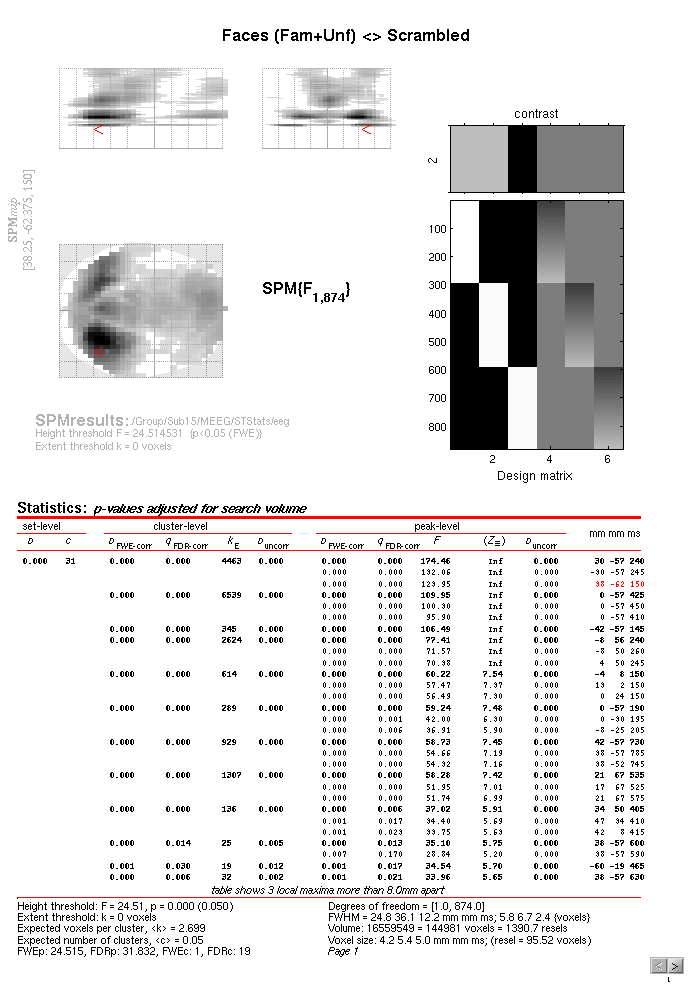
\includegraphics[width=150mm]{multi/figures/figure6}
\caption{\em Scalp-Time SPM for F-contrast, thresholded at p<.05 FWE corrected, for faces vs scrambled faces across trials for one subject. \label{multi:fig:6}}
\end{center}
\end{figure}

If you move the cursor to the earliest local maximum -- the third local peak in the first cluster -- this corresponds to \texttt{x=+38mm}, \texttt{y=-62mm} and \texttt{t=150ms} (i.e. right posterior scalp, close to the sensor shown in Figure~\ref{multi:fig:3}, though note that distances are only approximations). If you then press ``Plot -- Contrast Estimates -- All Effects'', you will get 6 bars like in Figure~\ref{multi:fig:7}. The first three reflect the three main conditions (the red bar is the standard error from the model fit). You can see that Famous and Unfamiliar faces produce a more negative amplitude at this space-time point than Scrambled faces (the ``N70''). The next three bars show the parameter estimates for the modulation of the evoked response by time. These effects are much smaller relative to their error bars (i.e., less significant), but suggest that the N170 to Famous faces becomes less negative with time, and that to scrambled faces becomes larger (though one can test these claims formally with further contrasts).

\begin{figure}
\begin{center}
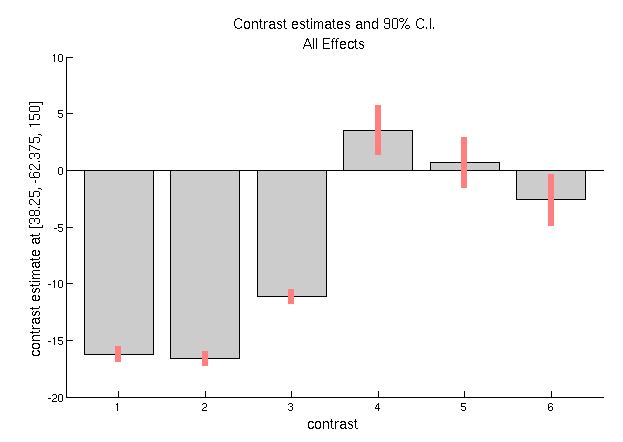
\includegraphics[width=100mm]{multi/figures/figure7}
\caption{\em Effects of interest from sub-peak +38mm -62mm +150ms. First three bars are mean evoked response amplitude vs baseline for Famous, Unfamiliar and Scrambled faces; next three bars are modulations about mean by time throughout experiment. \label{multi:fig:7}}
\end{center}
\end{figure}

There are many further options you can try. For example, within the bottom left window, there will be a section named ``Display'', in the second drop-down box, select ``Overlay -- Sections'' and from the browser, select the \texttt{mask.nii} file in the analysis directory. You will then get a clearer image of suprathreshold voxels within the scalp-time-volume. Or you can of course examine other contrasts, such as the difference between famous and unfamiliar faces, which you will see is a much weaker and slightly later effect.

\section{Time-Frequency Analysis (Evoked and Induced power)}

The above statistical test only identifies significant evoked effects (i.e., that are phase-locked across trials) within one individual. We can also look at induced as well as evoked energy by performing a time-frequency analysis before averaging over trials. Here we will use Morlet wavelets to decompose each trial into power and phase across peristimulus time and frequency. We will then average the power estimate across trials and across channels, to create a 2D time-frequency image, which we can then test for reliability, but now across subjects rather than across trials. This is the second fork in the preprocessing pipeline.

\subsection{Wavelet estimation}

The first module to be added to the pipeline is the ``Time-Frequency Analysis'' under ``SPM -- M/EEG -- Time-frequency''. Highlight ``File Name'', choose ``Specify'' box, and select the file \texttt{Mcbdspmeeg\_run\_01\_sss.mat}. This file has not yet been cropped because we need the 400ms buffer to reliably estimate the lower-frequency wavelets (in fact, for a 5-th order 6Hz wavelet, one needs 2.5 periods = 2.5\(\times\)133ms \(\sim\)400ms to reliably estimate power at the central timepoint). Note that this file does not have artifacts removed, but most of these identified for the evoked analysis above are blinks, which are typically below \(\sim\)3Hz, i.e., below the lowest frequency of interest here.

Next, ensure ``channel selection'' is set to ``all''. Then highlight the ``Frequencies of interest'', click ``Specify'' and enter \texttt{6:40} (which will estimate frequencies from 6 to 40Hz in steps of 1Hz). Then highlight ``Spectral estimation'' and select ``Morlet wavelet transform''. Then highlight ``Number of wavelet cycles'' and ``Specify'' this as \texttt{5}. The fixed time window length should be set at \texttt{0} as default. To reduce the size of the file, we will also subsample in time by a factor of 5 (i.e., every 25ms, given the additional downsampling to 5ms done earlier in preprocessing). Do this by selecting ``subsample'' and ``Specify'' as \texttt{5}. Finally, select ``Yes'' for ``Save phase''. This will produce two files, one for power (prefixed with \texttt{tf}) and one for phase (prefixed with \texttt{tph}).

\subsection{Crop}

Once we have estimated power and phase at every peristimulus timepoint, we can cut the 400ms buffer. So add the ``SPM -- M/EEG -- Preprocessing -- Crop'' module (like for the evoked analysis). This module will have to be added twice though, once for power and once for phase. For the first module, select the power file as the dependency, and enter \texttt{[-100 800]} as the timewindow. Then select ``replicate module'', and change only the input dependency to the phase file.

\subsection{Average}

As with cropping, we now need to add two averaging modules, one with dependency on the power file from the Crop step, and the other with dependency on the phase file from the Crop step. For the power averaging, choose straight averaging. For the phase averaging however, we need to additionally select ``Yes'' to the ``Compute phase-locking value''. This corresponds to ``circular'' averaging, because phase is an imaginary number. This produces a quantity called the phase-locking value (PLV). The prefix will be \texttt{m} in both cases. 

\subsection{Baseline rescaling}

To baseline correct time-frequency data, we need to select the ``Time-Frequency Rescale'' option from the ``Time-Frequency'' menu (note: not the ``Baseline Correction'' module from the ``Preprocessing'' menu). There are several options to baseline-correct time-frequency data. For the power, it also helps to scale the data with a log transform, because changes at high-frequency tend to be much smaller than changes at lower frequencies. We will therefore use the log-ratio (``LogR'') option, where all power values at a given frequency are divided by the mean power from -100 to 0ms at that frequency, and the log taken (which is equivalent to subtracting the log of the baseline power). So select the power file output from the previous phase as the dependency, select the log ratio option, and enter the baseline time window as \texttt{-100 0}. The output file prefix will be \texttt{r}. We won't bother to baseline-correct the phase-data.

\subsection{Contrasting conditions}

Finally, like with the evoked fork, we can take contrasts of our trial-averaged data, e.g., to create a time-frequency image of the difference in power, or in PLV, between faces and scrambled faces. Create two ``SPM -- M/EEG -- Average -- Contrast over epochs'' modules, one with the average power file as input, and one with the averaged phase (PLV) file as input. You can then select ``New Contrast'' and enter contrasts like \texttt{[0.5 0.5 -1]} (for faces vs scrambled; see earlier) and \texttt{[1 -1 0]} (for famous vs unfamiliar). The resulting output file is prepended with \texttt{w}.

As before, if you want to save file-space, you can add further ``Delete'' modules, since we will not need many of the intermediate files. The only files we need to keep are the averaged power and phase files (since these are used to create time-frequency images below) and the contrasted versions (for visual inspection of effects within each subject).

\paragraph{Save batch and review.}

You can now save this time-frequency batch file (it should look like the \texttt{batch\_preproc\_meeg\_tf\_job.m} file in the \texttt{SPM12batch} FTP directory). Once you have run it, you can then review the contrast files, e.g, for power (\texttt{wmprtf\_Mcbdspmeeg\_run\_01\_sss.mat}) or phase (\texttt{wmptph\_Mcbdspmeeg\_run\_01\_sss.mat}). When displaying the power for the EEG data, if you magnify Channel 70 (right posterior, as in Figure~\ref{multi:fig:3}), you should see something like that in Figure~\ref{multi:fig:8}. The increase in power from 13 to 16Hz between 75 and 200ms is most likely the evoked energy corresponding to the N170 in Figure~\ref{multi:fig:3}, but additional power changes can be seen that may not be so phase-locked (i.e. induced). This is supported by looking at the difference in PLV for that channel (Figure~\ref{multi:fig:9}), where faces increase phase-locking relative to scrambled faces in a similar time-frequency window (suggesting a change in phase of ongoing alpha oscillations, as well as their power).

\begin{figure}
\begin{center}
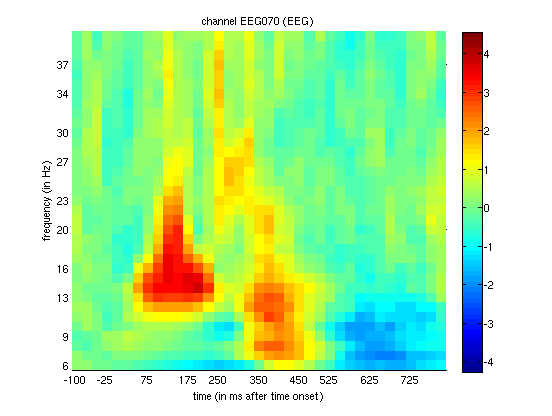
\includegraphics[width=100mm]{multi/figures/figure8}
\caption{\em Trial-averaged power for faces > scrambled in EEG channel 70 (right posterior). \label{multi:fig:8}}
\end{center}
\end{figure}

\begin{figure}
\begin{center}
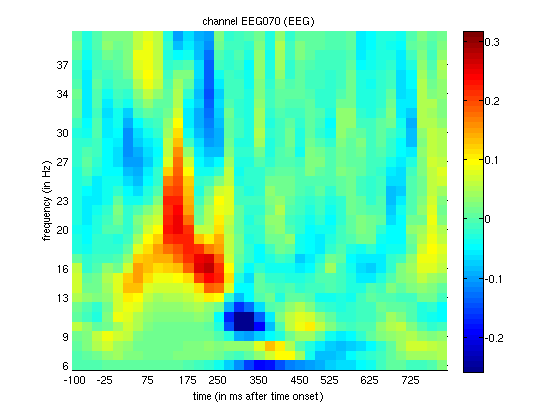
\includegraphics[width=100mm]{multi/figures/figure9}
\caption{\em Trial-averaged PLV for faces > scrambled in EEG channel 70 (right posterior). \label{multi:fig:9}}
\end{center}
\end{figure}

\subsection{Creating 2D time-frequency images}

Later we will repeat the above steps for every subject, and create a statistical parametric map of power changes across subjects, in order to localise face-induced power changes in frequency and time. This requires that we create 2D images, one per condition (per subject). Select the ``convert2images'' option and select the baseline-rescaled, trial-averaged power file as the dependency from the stage above. Select the mode ``time x frequency''. Note that this implicitly means averaging across all channels. Next select channel selection by type. Here, choose EEG for ``Channel selection'' and define the prefix as \texttt{eeg\_img\_pow}. (Of course, this module can be repeated for MEGMAG and MEGPLANAR   sensors  if wanted.) You can save this batch, run it, and display the images output if you like (the FTP batch is called \texttt{batch\_preproc\_meeg\_tf\_images\_job.m}).

\paragraph{Creating a script for analysis across subjects.}

Now that we have created pipelines for various steps of preprocessing one subject, including the two forks for evoked and time-frequency analyses, we want to run these on the remaining 15 subjects. For this, a bit of \matlab\ knowledge is required to call these pipelines within a \texttt{for} (or \texttt{parfor}) loop across subjects. Below is an example from the \texttt{master\_script.m}:

\begin{lstlisting}[style=Matlab-editor,basicstyle=\mlttfamily\footnotesize]
for s = 1:nsub
    
    %% Change to subject's directory
    swd = fullfile(outpth,subdir{s},'MEEG');
    cd(swd);
     
    %% Convert & epoch, prepare, downsample, baseline-correct each run   
    jobfile = {fullfile(scrpth,'batch_preproc_meeg_convert_job.m')};
    jobs    = repmat(jobfile, 1, nrun);
    n = 1;
    inputs  = cell(nrun*3, 1);
    for r = 1:nrun
        inputs{n  ,1} = cellstr(fullfile(rawpth,subdir{s},'MEEG',sprintf('run_%02d_sss.fif',r)));
        inputs{n+1,1} = cellstr(fullfile(rawpth,subdir{s},'MEEG','Trials',sprintf('run_%02d_trldef.mat',r)));
        inputs{n+2,1} = cellstr(fullfile(rawpth,subdir{s},'MEEG','bad_channels.mat'));
        n = n + 3;
    end
    spm_jobman('serial' , jobs, '', inputs{:});
    
    %% Concatenate runs and montage (reref EEG)
    jobfile = {fullfile(scrpth,'batch_preproc_meeg_merge_job.m')};   
    inputs  = cell(3, 1);
    inputs{1} = cellstr(spm_select('FPList',fullfile(outpth,subdir{s},'MEEG'),'^bdspmeeg.*\.mat$'));
    inputs{2} = cellstr(spm_select('FPList',fullfile(outpth,subdir{s},'MEEG'),'^bdspmeeg.*\.mat$'));  % (For deletion)  
    spm_jobman('serial', jobfile, '', inputs{:});

    %% Fork 1. For ERP/ERF: crop to -100 to +800, detect artifacts (blinks) by thresholding EOG, combine planar grads, average over trials and create contrasts of conditions
    jobfile = {fullfile(scrpth,'batch_preproc_meeg_erp_job.m')};
    inputs  = cell(1);
    inputs{1} = cellstr(spm_select('FPList',fullfile(outpth,subdir{s},'MEEG'),'^Mcbdspmeeg.*\.mat$'));
    spm_jobman('serial', jobfile, '', inputs{:})
    
    %% Write out scalp-time images
    if strcmp(subdir{s},'Sub15')
    jobfile = {fullfile(scrpth,'batch_preproc_meeg_erp_images_job.m')};
    inputs  = cell(3,1);
    inputs{1} = cellstr(spm_select('FPList',fullfile(outpth,subdir{s},'MEEG'),'^PapMcbdspmeeg.*\.mat$'));
    inputs{2} = cellstr(spm_select('FPList',fullfile(outpth,subdir{s},'MEEG'),'^PapMcbdspmeeg.*\.mat$'));
    inputs{3} = cellstr(spm_select('FPList',fullfile(outpth,subdir{s},'MEEG'),'^PapMcbdspmeeg.*\.mat$'));
    spm_jobman('serial', jobfile, '', inputs{:});
    end

    %% Fork 2. For Time-freq: Morlet wavelet transform, crop, average, baseline-correct (power) and contrast   
    jobfile = {fullfile(scrpth,'batch_preproc_meeg_tf_job.m')};
    inputs  = cell(1);
    inputs{1} = cellstr(spm_select('FPList',fullfile(outpth,subdir{s},'MEEG'),'^Mcbdspmeeg.*\.mat$'));
    spm_jobman('serial', jobfile, '', inputs{:});

    %% Write out power and phase images for each modality
    jobfile = {fullfile(scrpth,'batch_preproc_meeg_tf_images_job.m')};
    inputs  = cell(6,1);
    inputs{1} = cellstr(spm_select('FPList',fullfile(outpth,subdir{s},'MEEG'),'^mprtf_Mcbdspmeeg.*\.mat$'));
    inputs{2} = cellstr(spm_select('FPList',fullfile(outpth,subdir{s},'MEEG'),'^mprtf_Mcbdspmeeg.*\.mat$'));
    inputs{3} = cellstr(spm_select('FPList',fullfile(outpth,subdir{s},'MEEG'),'^mprtf_Mcbdspmeeg.*\.mat$'));
    inputs{4} = cellstr(spm_select('FPList',fullfile(outpth,subdir{s},'MEEG'),'^mptph_Mcbdspmeeg.*\.mat$'));
    inputs{5} = cellstr(spm_select('FPList',fullfile(outpth,subdir{s},'MEEG'),'^mptph_Mcbdspmeeg.*\.mat$'));
    inputs{6} = cellstr(spm_select('FPList',fullfile(outpth,subdir{s},'MEEG'),'^mptph_Mcbdspmeeg.*\.mat'));
    spm_jobman('serial', jobfile, '', inputs{:});

end
\end{lstlisting}

\paragraph{Time-frequency Stats across Subjects}

We can now enter the frequency-time power images (one per condition per subject) into a group (2nd-level) analysis that corresponds to repeated-measures ANOVA. Note that one difference from the ANOVA used for scalp-time analysis across trials within one subject above is that we now have 3 observations (conditions) from each subject, so need to correct for the potential correlation (nonsphericity) of the error induced by these repeated measurements. We can also add another 16 columns into our GLM that serve to remove between-subject variance (which we don't care about), improving the sensitivity of contrasts of our conditions of interest.

The first thing is to specify the output directory where the SPM stats files will be saved. Because this is now an analysis across subjects, we can create a directory above \texttt{Sub15} in the directory tree. So create a new top-level directory called, for example, ``MEEG'' (because later we will have group stats for the fMRI data and source-reconstructed MEEG data too), then a sub-directory within it called \texttt{TFStats}, and then a further sub-directory called \texttt{PowStats} and a further sub-directory called \texttt{eeg} (and potentially two more called \texttt{mag} and \texttt{grd} if you want to examine other sensor-types too).

\subsection{Model Specification, Estimation and Contrasts}

To create this repeated-measures ANOVA, open a new batch and select ``Factorial design specification'' under ``Stats'' on the ``SPM'' toolbar. Then select this new \texttt{MEEGTFStats/PowStats/eeg} directory.

Highlight ``Design'' and from the current item window, select ``One-way ANOVA --within subject'' (somewhat confusingly, this is not an analysis within one subject, as above, but an analysis in which multiple measures come from ``within'' each subject!). Highlight ``Subjects'' and create a ``New:subject''. In the ``scans'' field, you can now select the 3 power images for the first subject (which should have been created in the \texttt{Sub01/MEEG/eeg\_img\_pow\_mprtf\_Mcbdspmeeg\_run\_01\_sss} directory if you ran the script above), and enter the ``Conditions'' as \texttt{[1 2 3]}. It is important for the contrasts below that you select the files in the order Famous-Unfamiliar-Scrambled (or if not, that you change the order of 1-3 in the Conditions vector, such that Condition 1 is Famous, Condition 2 Unfamiliar, etc.). You can then select ``Replicate: Subject'' under the ``Subjects'' item, keeping the ``Conditions'' unchanged, but changing the ``Scans'' to those in \texttt{Sub02/MEEG/eeg\_img\_pow\_mprtf\_Mcbdspmeeg\_run\_01\_sss}. You can then repeat these steps for the remaining subjects. Or if you prefer (because this is a pain to do via the GUI!), you can create 16 blank ``Subject'' items, save the batch script, and then populate the ``Scans'' field (and Conditions field) via a \matlab\ script (see below). Finally, set the variance to ``Unequal'' and the ``Independence'' to ``No'' (to model the error correlation, i.e., nonsphericity, mentioned above). Keep all the remaining defaults. 

The next step is to add a module for model estimation from the ``Stats'' option and define the file name as being dependent on the results of the factorial design specification output. For ``write residuals'', keep ``no''. Select classical statistics. 

The final step is to add a module for creating contrasts. Define the file name as dependent on the model estimation. The first contrast will be a generic one that tests whether significant variance is captured by the first 3 regressors. This corresponds to an F-contrast based on a 3\(\times\)3 identity matrix. Highlight contrast sessions and select a new F-contrast session, using the current item module. Name this contrast ``All Effects''. Then define the weights matrix by typing in \texttt{[eye(3) ones(3,16)/16]} (which is \matlab\ for a 3\(\times\)3 identity matrix, followed by \texttt{1/16} for each of the 16 subject effects; the latter being necessary if one wants to see absolute changes in power vs baseline). You can use this contrast later to plot the parameter estimates for the 3 conditions.

More interestingly perhaps, we can also define a contrast that compares faces against scrambled faces, i.e., to test whether the average power increase across trials seen in Channel 70 of Subject 15 in Figure~\ref{multi:fig:8} is reliable when averaging across channels and across subjects. So this time make a T-contrast, name this one ``Faces (Fam+ Unf) \(>\) Scrambled'', and type in the weights \texttt{[0.5 0.5 -1]}. (If you want to look at power decreases, you can create another T-contrast and reverse the sign of these contrast weights.)

\paragraph{Save batch and review}

Once you had added all the contrasts you want, you can save this batch file (it should look like the \texttt{batch\_stats\_rmANOVA\_job.m} file in the \texttt{SPM12batch} FTP directory). Then run it, and when it has finished, press ``Results'' from the SPM Menu window. Select the \texttt{SPM.mat} file in the \texttt{MEEG/TFStats/eeg} directory, and from the new Contrast Manager window, select the pre-specified T-contrast ``Faces (Fam+Unf) \(>\) Scrambled''.  Within the Interactive window, when given the option, select the following:  Apply Masking: None, P value adjustment to control: FWE, keep the threshold at 0.05, extent threshold {voxels}: 0; Data Type: Time-frequency. The Graphics window should then show what is in Figure 10 below.  Note the increase in power at ~14Hz, 150ms that survives correction (in all sensor types in fact). (If you examine the reverse contrast of greater power for scrambled than intact faces, you will see a decrease in the beta range, ~22Hz, 475ms).

\begin{figure}
\begin{center}
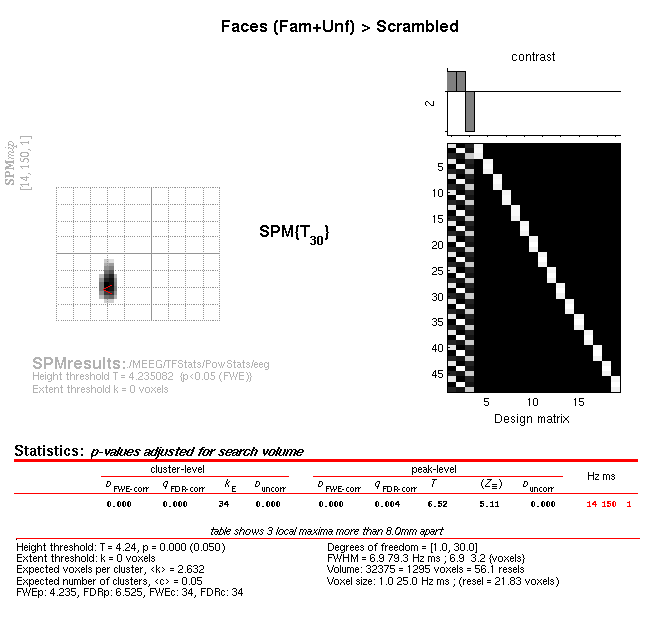
\includegraphics[width=120mm]{multi/figures/figure10}
\caption{\em Time-Frequency SPM for T-contrast of greater power for faces than scrambled faces across subjects, thresholded at \(p<.05\) FWE corrected. \label{multi:fig:10}}
\end{center}
\end{figure}

\section{fMRI Preprocessing and Statistics}

We will keep description of the preprocessing and analysis of the fMRI data to a minimum, given that fMRI analysis is covered in several other chapters. We start with preprocessing Subject 15's data. For the fMRI experiment, there were 9 runs (sessions), rather than the 6 in the M/EEG experiment. This is because the SOA was increased in the fMRI experiment, by virtue of jittering, which is necessary to estimate the BOLD response versus interstimulus baseline (e.g., to compare with the evoked EEG/MEG response versus prestimulus baseline). If you already launched SPM to analyse the M/EEG data from the previous sections, select ``FMRI'' instead of ``EEG'' in the pulldown menu of the main SPM window, otherwise start SPM by typing \texttt{spm fmri}. Preprocessing involves the following modules, which can be found under the menu ``SPM -- Spatial'':

\subsection{Realignment of EPI (fMRI) data}

The first step is to coregister the 9 runs of 208 images to one another (i.e., correcting for movement) using a rigid-body transform. Select ``Realign: Estimate \& Reslice'', and on the ``Data'' item, add nine new ``Sessions''. Then, for the first session, select the 208 \texttt{f*.nii} images in the \texttt{BOLD/Run\_01} directory of Subject 15 (using right-click, ``Select All''), and then repeat for the remaining eight sessions. On the ``Reslice Options'' item, change the default value of ``All Images + Mean Image'' to ``Mean Image Only''. This is because we do not re-slice the EPI data: the coregistration parameters will be stored in the header information of the NIfTI file, and can be combined with the normalisation parameters when re-slicing the normalised images below (re-slicing can introduce interpolation artifacts so generally best to reduce number of re-slicings). However, we do need a re-sliced mean image, which we can use for coregistration with the T1 below. Thus the contents of the \texttt{f*.nii} files will change (as header updated), but no new (\texttt{rf*.nii}) files will be output, except for the \texttt{meanf*.nii} file.

\subsection{Normalisation/Segmentation of T1 images}

We will use SPM12's unified segmentation to estimate normalisation parameters to MNI space. Select ``Normalise: Estimate'' item, add a new ``Subject'' in ``Data'' and select the \texttt{mprage.nii} image in the ``SMRI'' directory of Subject 15 for ``Image to Align''. The output of this step will be a file \texttt{y\_mprage.nii} containing the estimated deformation field that warps data from subject to MNI space.

\subsection{Coregistration of mean EPI (fMRI) to T1 (sMRI)}

Because we have determined the normalisation parameters from the subject's native space to MNI space via the unified segmentation of their T1 image, we need to coregister all the EPI images to that T1 image, so that the normalisation warps can be later applied. Select ``Coregister - Estimate'' item, and for the ``Reference Image'', select the same \texttt{mprage.nii} image in the \texttt{SMRI} directory. For the``Source Image'', select ``Dependency'' and then use ``Realign: Estimate \& Reslice: Mean Image''. For ``Other Images'', select ``Dependency'' and then use the Ctrl key to select all 9 sessions from the ``Realign'' stage.

\subsection{Application of Normalisation parameters to EPI data}

We can now apply the normalisation parameters (warps) to each of the EPI volumes, to produce new, re-sliced \texttt{wf} images. Select ``Normalise -- Write'' item, and for the ``Deformation Field'', use select the ``Normalise: Estimate: Deformation'' dependency. For the ``Images to Write'', select the ``Coregister: Estimate: Coregistered Images''. You can also change the default voxel size from \texttt{[2 2 2]} to \texttt{[3 3 3]} if you want to save diskspace, since the original data are [3 3 3.9] (for Subject 15), so interpolation does not really gain new information.

\subsection{Smoothing}

Finally, we smooth the normalised images by an 8mm isotropic Gaussian kernel to produce \texttt{swf*} images. So select the ``Smooth'' item, and select the input to depend on the output of the prior ``Normalisation: Write'' stage.

\paragraph{Save batch and review}

You can save this batch file (it should look like the \texttt{batch\_preproc\_fmri\_job.m} file in the \texttt{SPM12batch} FTP directory), and then run it. You can inspect the realignment parameters, normalisations, etc. as described in other chapters. Make a new directory called \texttt{Stats} in the \texttt{Sub15/BOLD} directory.

\subsection{Creating a 1st-level (fMRI) GLM}

Select the ``fMRI model specification'' option from the ``SPM -- Stats'' menu. Select the new \texttt{Stats} directory you created as the output directory. Set the ``Units for design'' to ``seconds'' (since our onsets files are in units of seconds) and the ``interscan interval'' (TR) to \texttt{2}. Then under the ``Data \& Design'' option, create a new Session, and then select all the \texttt{swf*.nii} images in the \texttt{Run\_01} directory as the ``Scans''. Then under the ``Multiple conditions'' option, press ``Specify'' and select the file \texttt{run\_01\_spmdef.mat} that has been provided in the \texttt{Trials} sub-directory. This is a \matlab\ file that contains the onsets, durations and names of every trial in \texttt{Run1} (for this subject). Then under the ``Multiple regressors'' option, press ``Specify'' and select the file matching \texttt{rp*.txt} in the \texttt{Run\_01} directory. This is a text file that contains the 6 movement parameters for each scan, which was created during ``Realignment'' above, and we will add to the GLM to capture residual motion-related artifacts in the data.

For the basis functions, keep ``Canonical HRF'', but change the ``model derivatives'' from ``no'' to ``time and dispersion derivatives'' (see earlier Chapter manuals). Then keep the remaining options as their defaults.

You then need to replicate this for the remaining 8 sessions, updating all three fields each time: i.e., the scans, conditions and (movement) regressors. It is at this point, that you might want to switch to scripting, which is much less effort -- see e.g. this:

\begin{lstlisting}[style=Matlab-editor,basicstyle=\mlttfamily\footnotesize]
swd = '.../Sub15/BOLD'; % folder containing Subject 15's fMRI data
clear matlabbatch
matlabbatch{1}.spm.stats.fmri_spec.dir = {fullfile(swd,'Stats')};
matlabbatch{1}.spm.stats.fmri_spec.timing.units = 'secs';
matlabbatch{1}.spm.stats.fmri_spec.timing.RT = 2;
for r=1:9
    matlabbatch{1}.spm.stats.fmri_spec.sess(r).scans = ...
        cellstr(spm_select('FPList',fullfile(swd,sprintf('Run_%02d',r)),'^swf.*\.nii'));
    matlabbatch{1}.spm.stats.fmri_spec.sess(r).multi = ...
        cellstr(fullfile(swd,'Trials',sprintf('run_%02d_spmdef.mat',r)));
    matlabbatch{1}.spm.stats.fmri_spec.sess(r).multi_reg = ...
        cellstr(spm_select('FPList',fullfile(swd,sprintf('Run_%02d',r)),'^rp_.*\.txt'));
end
matlabbatch{1}.spm.stats.fmri_spec.bases.hrf.derivs = [1 1];
spm_jobman('interactive',matlabbatch);
\end{lstlisting}

\subsection{Model Estimation}

Add a module for ``Model estimation'' from the ``SPM -- Stats'' menu and define the \texttt{SPM.mat} file name as being dependent on the results of the fMRI model specification output. For ``write residuals'', keep ``No'' and stick to ``Classical'' estimation.

\subsection{Setting up contrasts}

To create some contrasts, select ``Contrast Manager'' from the ``SPM -- Stats'' menu. Define the \texttt{SPM.mat} file name as dependent on the model estimation. The first contrast will be a generic one that tests whether significant variance is captured by the 3 canonical HRF regressors (one per condition). So create a new F-contrast, call it the ``Canonical HRF effects of interest'', and enter as the weights matrix (SPM will automatically perform zero padding over the movement regressors):
\begin{verbatim}
   [1 0 0 0 0 0 0 0 0
    0 0 0 1 0 0 0 0 0
    0 0 0 0 0 0 1 0 0]
\end{verbatim}
Then select ``Replicate'' to reproduce this across the 9 sessions. We can also define a T-contrast to identify face-related activation, e.g., ``Faces \(>\) Scrambled Faces'', given the weight matrix \texttt{[0.5 0 0  0.5 0 0  -1 0 0]}, again replicated across sessions. (Note that there are 3 basis functions per condition, and the zeros here ignore the temporal and dispersion derivatives, but if you want to include them, you can add them as separate rows and test for any face-related differences in BOLD response with an F-contrast; see earlier chapters).

Finally, for the group-level (2nd-level) analyses below, we need an estimate of activation of each condition separately (versus baseline), averaged across the sessions. So create three new T-contrasts, whose weights correspond to the three rows of the above F-contrast, i.e, that pick out the parameter estimate for the canonical HRF (with ``Replicate over sessions'' set to ``Replicate''):

\begin{itemize}
    \setlength\itemsep{0em}
	\item[] for Famous: \texttt{[1 0 0 0 0 0 0 0 0]},
	\item[] for Unfamiliar: \texttt{[0 0 0 1 0 0 0 0 0]},
	\item[] for Scrambled: \texttt{[0 0 0 0 0 0 1 0 0]}.
\end{itemize}

These T-contrasts will be numbered 3-5, and used in group analysis below.\footnote{
Note that you can create a \matlab\ variable containing the weights of the F-contrast with \texttt{C = kron(eye(3),[1 0 0])}, and then enter \texttt{C}, \texttt{0.5*C(1,:)+0.5*C(2,:)-C(3,:)}, \texttt{C(1,:)}, \texttt{C(2,:)} and \texttt{C(3,:)} respectively for the 5 contrasts specified above.
}

\paragraph{Save batch and review}

You can save this batch file (it should look like the \texttt{batch\_stats\_fmri\_job.m} file in the \texttt{SPM12batch} FTP directory). When it has run, you can press ``Results'' from the SPM Menu window, select the \texttt{SPM.mat} file in the \texttt{BOLD} directory, and explore some of the contrasts. However, we will wait for the group analysis below before showing results here.

\paragraph{Creating a script for analysis across subjects}

Now that we have created a pipeline for fMRI preprocessing and analysis for a single subject, we can script it to run on the remaining 15 subjects. Below is an example from the \texttt{master\_script.m}:

\begin{lstlisting}[style=Matlab-editor,basicstyle=\mlttfamily\footnotesize]
nrun = 9;

spm_jobman('initcfg');
spm('defaults', 'FMRI');
for s = 1:nsub
    
    %% Change to subject's directory
    swd = fullfile(outpth,subdir{s},'BOLD');
    cd(swd);
    
    %% Preprocessing
    jobfile = {fullfile(scrpth,'batch_preproc_fmri_job.m')};
    inputs  = cell(nrun+2,1);
    for r = 1:nrun
        inputs{r} = cellstr(spm_select('FPList',fullfile(outpth,subdir{s},'BOLD',sprintf('Run_%02d',r)),'^fMR.*\.nii$'));
    end   
    inputs{10} = cellstr(spm_select('FPList',fullfile(outpth,subdir{s},'SMRI'),'^mprage.*\.nii$'));
    inputs{11} = cellstr(spm_select('FPList',fullfile(outpth,subdir{s},'SMRI'),'^mprage.*\.nii$'));
    spm_jobman('serial', jobfile, '', inputs{:});
    
    %% 1st-level stats
    jobfile = {fullfile(scrpth,'batch_stats_fmri_job.m')};
    inputs  = {}; %cell(nrun*3+1,1);
    inputs{1} = {fullfile(swd,'Stats')}; 
    try mkdir(inputs{1}{1}); end
    for r = 1:nrun
        inputs{end+1} = cellstr(spm_select('FPList',fullfile(outpth,subdir{s},'BOLD',sprintf('Run_%02d',r)),'^swfMR.*\.nii$'));
        inputs{end+1} = cellstr(fullfile(outpth,subdir{s},'BOLD','Trials',sprintf('run_%02d_spmdef.mat',r)));
        inputs{end+1} = cellstr(spm_select('FPList',fullfile(outpth,subdir{s},'BOLD',sprintf('Run_%02d',r)),'^rp.*\.txt$'));
    end   
    spm_jobman('serial', jobfile, '', inputs{:});

    eval(sprintf('!rm -r %s/Run*/f*',swd)) % to save diskspace (take care!)
    eval(sprintf('!rm -r %s/Run*/wf*',swd)) % to save diskspace (take care!)
end
\end{lstlisting}

(The last two lines in the loop are optional, to delete intermediate files and save diskspace.) 
Once you have run this script, we can do 2nd-level (group) statistics on resulting contrast images for each condition (averaged across 9 runs).

\subsection{Group Statistics on fMRI data}

Now we have a new set of 16\(\times\)3 NIfTI images for each subject and each condition, we can put them into the same repeated-measures ANOVA that we used to test for differences in power across sensors in the time-frequency analysis above, i.e, re-use the \texttt{batch\_stats\_rmANOVA\_job.m} file created above. This can be scripted as:

\begin{lstlisting}[style=Matlab-editor,basicstyle=\mlttfamily\footnotesize]
fmristatsdir = fullfile(outpth,'BOLD');
if ~exist(fmristatsdir)
    eval(sprintf('!mkdir %s',fmristatsdir));
end

jobfile = {fullfile(scrpth,'batch_stats_rmANOVA_job.m')};

inputs  = cell(nsub+1, 1);
inputs{1} = {fmristatsdir};
for s = 1:nsub
    inputs{s+1,1} = cellstr(strvcat(spm_select('FPList',fullfile(outpth,subdir{s},'BOLD','Stats'),'con_000[345].nii')));   % Assumes that these T-contrasts in fMRI 1st-level models are famous, unfamiliar, scrambled (averaged across sessions)
end

spm_jobman('serial', jobfile, '', inputs{:});
\end{lstlisting}

\paragraph{Save batch and review.}

When the script has run, press ``Results'' from the SPM Menu window and select the \texttt{SPM.mat} file in the \texttt{BOLD} directory. From the Contrast Manager window, select the pre-specified T-contrast ``Faces (Fam+Unf) \(>\) Scrambled''.  Within the ``Stats: Results'' window, when given the option, select the following:  Apply Masking: None, P value adjustment to control: FWE, keep the threshold at 0.05, extent threshold {voxels}: 0; Data Type: Volumetric 2D/3D. The Graphics window should then show what is in Figure~\ref{multi:fig:11} below. Note the left and right OFA and FFA (more extensive on right), plus a small cluster in left medial temporal lobe.

\begin{figure}
\begin{center}
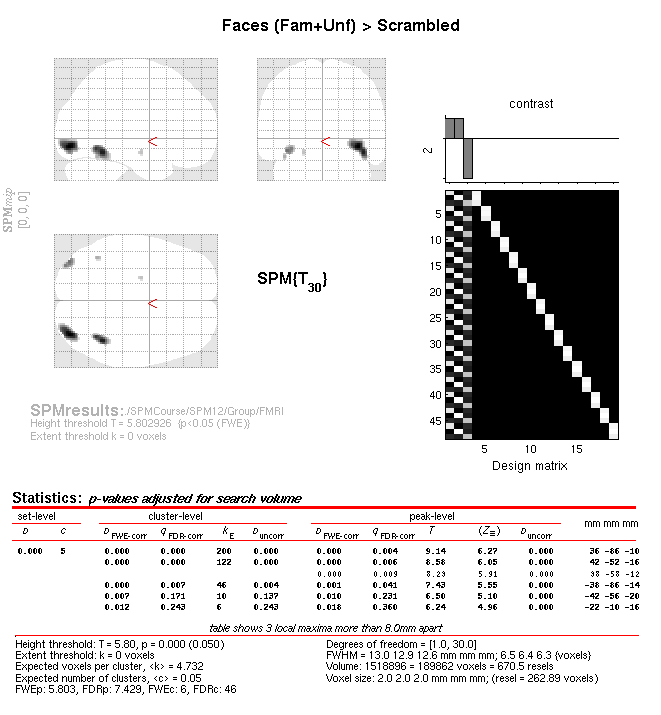
\includegraphics[width=100mm]{multi/figures/figure11}
\caption{\em Group SPM for Faces vs Scrambled fMRI data at \(p<.05\) FWE-corrected. \label{multi:fig:11}}
\end{center}
\end{figure}

Later, we can use these five clusters as priors for constraining the inversion of our EEG/MEG data. To do this, we need to save these as an image. Press the ``save...'' button in the bottom right of the SPM Results window, and select the ``all clusters (binary)'' option. The window will now prompt you for an output filename, in which you can type in \texttt{fac-scr\_fmri\_05\_cor}. This image will be output in the \texttt{BOLD} directory, and we will use it later.

\section{Source Reconstruction}

To estimate the cortical sources that give rise to the EEG and MEG data, we will return to Subject 15, in order to demonstrate forward and inverse modelling. We need to use the structural MRI of the subject to create a ``head model'' (that defines the cortex, skull and scalp in terms of meshes) and then a ``forward model'' (that uses a conductor model to simulate the signal at each sensor predicted by a dipolar source at each point in the cortical mesh). This corresponds to an ``imaging'' or ``distributed'' solution to the ``Inverse problem'', but you should note that SPM offers other inverse solutions, such as a Bayesian implementation of Equivalent Current Dipoles, and also DCM, which can be viewed as a type of inverse solution (see other chapters in this manual).

You can view the structural MRI of Subject 15 by displaying the NIfTI file \texttt{mprage.nii} in the \texttt{SMRI} (T1) sub-directory. This image was manually positioned to roughly match Talairach space, with the origin close to the Anterior Commissure. The approximate position of 3 fiducials within this MRI space -- the nasion, and the left and right pre-auricular points -- are stored in the file \texttt{mri\_fids.mat}. These were identified manually (based on anatomy) and are used to define the MRI space relative to the EEG and MEG spaces, which need to be coregistered (see below).

To estimate total power (evoked and induced) of the cortical sources, we need to have the original data for each individual trial. Therefore our input file will be \texttt{apMcbdspmeeg\_run\_01\_sss.mat} (we could select the trial-averaged file if we just wanted to localise evoked effects). Note that one cannot localise power (or phase) data directly, nor can one localise RMS data from combined gradiometers.

\subsection{Create Head Model}

Select the source reconstruction option in the batch window, and select ``Head model specification''. Select the file \texttt{apMcbdspmeeg\_run\_01\_sss.mat} as the ``M/EEG datasets'', and the inversion index as \texttt{1} (this index can track different types of forward models and inverse solutions, for example if you want to compare them in terms of log-evidence, e.g., Henson et al, 2009). Additional comments relating to each index can be inserted if ``comments'' is selected. 

The next step is to specify the meshes. Highlight ``meshes'' and select ``mesh source''. From here select ``Individual structural image'' and select the \texttt{mprage.nii} in the \texttt{SMRI} directory. The mesh resolution can be kept as normal (approximately 4000 vertices per hemisphere). Note that the cortical mesh (and scalp and skull meshes) are created by warping template meshes from a brain in MNI space, based on normalising this subject's MRI image to that MNI brain (see papers on ``canonical'' meshes in SPM).

To coregister the MRI and MEEG data, you must select ``specify coregistration parameters''. First you need to specify the select fiducials. You will need to select at least three of these, with coordinates in the space of the MRI image selected. Here we will define ``Nasion''; ``LPA''; ``RPA''. You can do this by loading the MRI and clicking, but here we will use the coordinates provided in the \texttt{mri\_fids.mat} file described above. You can view these coordinates by loading that file into \matlab\, but we repeat them below for convenience. For the Nasion, select ``type MRI coordinates'' and enter: \texttt{[4 112 1]}; for LPA, enter \texttt{[-80 21 -12]}; for RPA, enter \texttt{[79 9 -31]}.

As well as the fiducials, a number of ``head-points'' across the scalp were digitised. These were read from the FIF file and stored in the SPM MEEG file. These can help coregistration, by fitting them to the scalp surface mesh (though sometimes they can distort coregistration, e.g. if the end of the nose is digitised, since the nose does not appear on the scalp mesh, often because it has poor contrast on T1-weighted MRI images). If you keep ``yes'' for the ``use headshape points'' option, these points will be used, but you will notice that alignment of the fiducials is not as good (as if you don't use the headshape points), most likely because the nose points are pulling it too far forward. So here we will say ``no'' to the ``use headshape points'' option, so as to rely on the fiducials alone, and trust the anatomical skills of the experimenter. (Alternatively, you could edit the headpoints via the command line or a script so as to remove inappropriate ones, but we will not go into the details here).

Finally, for the forward model itself, select ``EEG head model'', and specify this as ``EEG BEM''; select ``MEG head model'' and specify this as ``Single Shell''. This can then be run. Note that the model parameters are saved, but the gain matrix itself is not estimated until inversion.

\paragraph{Save batch and review.}

You can now save this inversion batch file (it should look like the \texttt{batch\_localise\_forward\_model\_meeg\_job.m} file in the \texttt{SPM12batch} FTP directory). Once you have run it, you can explore the forward model by pressing the ``3D Source Reconstruction'' button within the SPM Menu window. This will create a new window, in which you can select ``Load'' and choose the \texttt{apMcbdspmeeg\_run\_01\_sss.mat} file.  On the left hand side of the ``source localisation'' window, select the ``display'' button below the ``MRI'' button. This will bring up the scalp (orange), inner and outer skull (red) and cortical (blue) meshes of Subject 15's brain, like in Figure~\ref{multi:fig:12} (left, after rotating slightly with \matlab\ 's 3D tool). Note that the fiducials are shown by cyan disks. 

\begin{figure}
\begin{center}
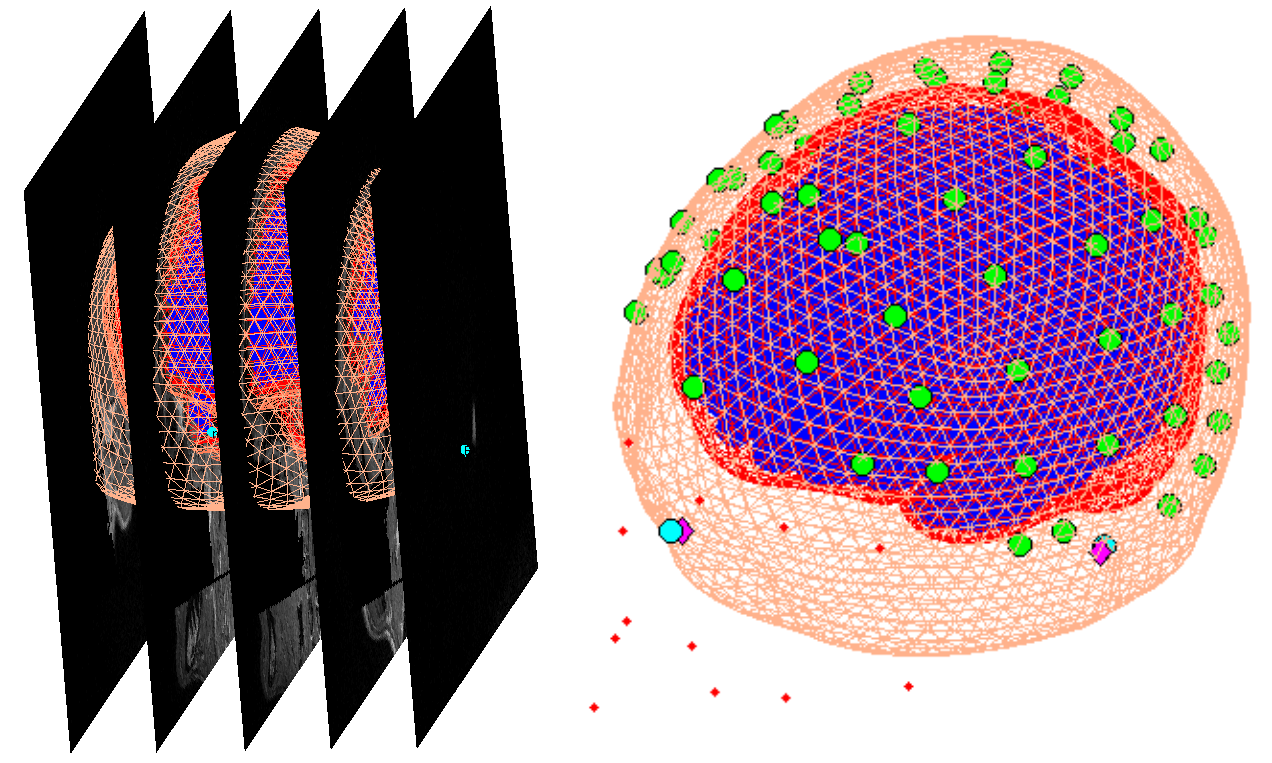
\includegraphics[width=100mm]{multi/figures/figure12}
\caption{\em Coregistration of meshes with MRI (left) and meshes with MEG (right). \label{multi:fig:12}}
\end{center}
\end{figure}

Next, select the ``display'' button beneath ``Co-register'' and then select ``EEG'' when asked  what to display. The Graphics window should then display an image like in Figure 12 (right) that displays the electrode locations in green disks, the digitized headpoints in small red dots, the fiducials in the EEG data as purple diamonds, and the MRI fiducials as cyan disks again. The overlap between the EEG fiducials and MRI fiducials indicates how well the data have been coregistered (assuming no error in marking these anatomical features). 

Finally, select ``Display'' located beneath ``Forward Model'' and this time select ``EEG''. You should see an image displaying the EEG electrode locations relative to the four meshes. 

\subsection{Model Inversion}

We will compare two approaches to inverting the above forward model (both within a Parametric Empirical Bayesian framework). The first one is called ``Multiple Sparse Priors'', which is a novel approach unique to SPM. This corresponds to a sparse prior on the sources, namely that only a few are active. Go back to the batch editor, and select ``M/EEG -- Source reconstruction -- Source Inversion''. Select the same input file \texttt{apMcbdspmeeg\_run\_01\_sss.mat}, and set the inversion index to \texttt{1}. Highlight ``what conditions to include'' and select ``All''. Next highlight inversion parameters, choose ``custom'' and set the inversion type to ``GS''. This is one of several fitting algorithms for optimising the MSP approach: Greedy Search (GS), Automatic Relevance Detection (ARD) and GS+ARD. We choose GS here because it is quickest and works well for these data. Then enter the time window of interest as \texttt{[-100 800]}. Set the frequency window of interest to \texttt{[0 256]}. Select ``yes'' for the ``PST Hanning window''. Keep all the remaining parameters at their defaults, including the Modalities as ``All'' (which will simultaneously invert, or ``fuse'', the data from the EEG, magnetometers and gradiometers [Henson et al, 2009]).

The second type of inversion we will examine corresponds to a L2-minimum norm (MNM), i.e, fitting the data at the same time as minimising the total energy of the sources. In SPM, this is called ``IID'' because it corresponds to assuming that the prior probability of each source being active is independent and identically distributed (i.e., an identity matrix for the prior covariance). Go back to the batch editor, add another ``M/EEG -- Source reconstruction -- Source Inversion'' module, and select the same input files as before (\texttt{apMcbdspmeeg\_run\_01\_sss.mat}), but this time set the inversion index to \texttt{2}. Set the inversion parameters to ``custom'', but the inversion type to be ``IID''. The remaining parameters should be made to match the MSP (GS) inversion above.

\subsection{Time-frequency contrasts}

Here we are inverting the whole epoch from -100 to +800ms (and all frequencies), which will produce a timecourse for every single source. If we want to localise an effect within the cortical mesh, we need to summarise this 4D data by averaging power across a particular time-frequency window. To do this, select ``M/EEG -- Source reconstruction -- Inversion Results''. Specify the input as dependent on the output of the source inversion, and set the inversion index to \texttt{1}. Based on the results of the group sensor-level time-frequency analyses in the previous section, set the time window of interest to \texttt{[100 250]} and the frequency window of interest to \texttt{[10 20]}. For the contrast type, select ``evoked'' from the current item window, and the output space as ``MNI''. Then replicate this module to produce a second ``inversion results'' module, simply changing the index from \texttt{1} to \texttt{2} (i.e. to write out the time-frequency contrast for the MNM (IID) as well as MSP (GS) solution).

Now the source power can be written in one of two ways: 1) either as a volumetric NIfTI ``Image'', or as 2) a surface-based GIfTI ``Mesh''. The source data are currently represented on the cortical mesh, so writing them to a volumetric image involves interpolation. If we chose this, we could treat the resulting contrast images in the same way that we do MRI images, and use 3D Random Field Theory (RFT) for voxel-wise statistics. This is likely to require considerable 3D smoothing however, to render the interpolated cortical surface more suitable for RFT. This is what was done in SPM8. However, in SPM12, RFT can also be applied to 2D surfaces (that live in a 3D space), in which case we can restrict smoothing to a small amount across the surface (rather than volume), which is closer to the nature of the data. Therefore, we will chose ``Mesh'' here to write out GifTI surfaces (which are also much smaller in filesize), keeping the default cortical smoothing of \texttt{8}.

\paragraph{Save batch and review}

You can now save this inversion batch file (it should look like the \texttt{batch\_localise\_evoked\_job.m} file in the \texttt{SPM12batch} FTP directory). It will take a while to run (because it has to create the gain matrix for the first time), after which you can review the inverse results from within the same ``3D Source Reconstruction'' interface that you used to examine the forward model above. You have to re-``Load'' the \texttt{apMcbdspmeeg\_run\_01\_sss.mat} file. The latest inversion index will be shown (2 in this case), which corresponds to the IID inversion. Press the ``mip'' button below the ``Invert'' button, and you should see something like Figure~\ref{multi:fig:13}. The top plot shows the evoked responses for the three conditions from the peak vertex (at +52 -59 -21, i.e. right fusiform) at 165ms, with the red line being the currently selected condition, here ``1'' for Famous faces (press the ``condition'' button to toggle through the other conditions). If you press ``display'' under the ``Window'' button, you can see a MIP for the time-frequency contrast limited to the 100-250ms, 10-20Hz specified above, or if you press the ``display'' under the ``Image'' button, you will see a rendered version.

\begin{figure}
\begin{center}
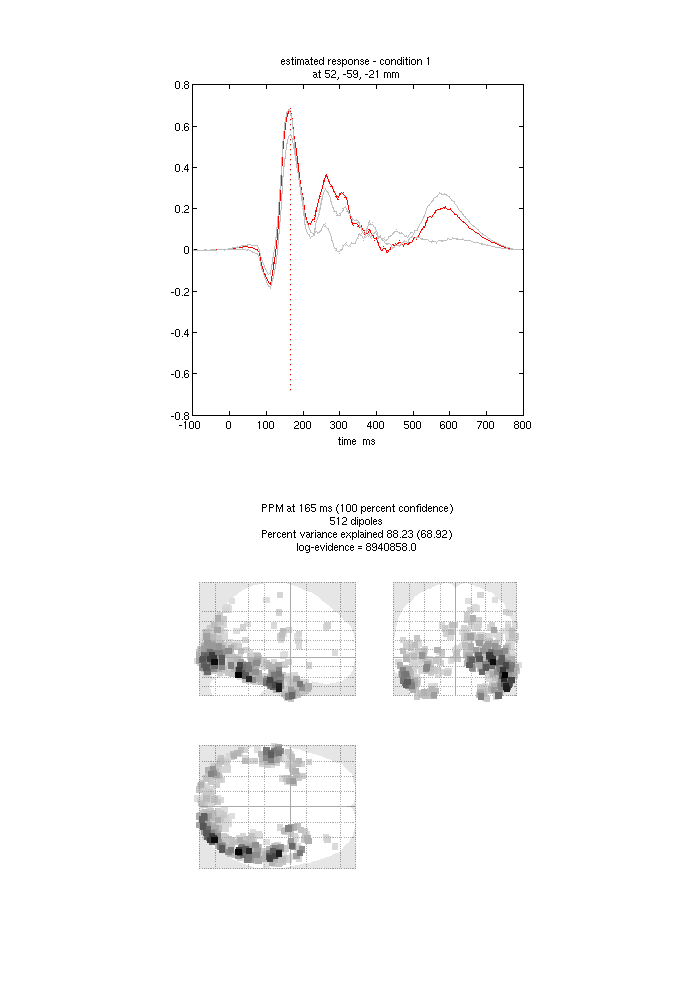
\includegraphics[width=150mm]{multi/figures/figure13}
\caption{\em Maximal Intensity Projection (MIP) for Minimum Norm (IID) inversion of Subject 15’s fused EEG and MEG data. \label{multi:fig:13}}
\end{center}
\end{figure}

If you press the ``previous'' button, you can select the previous inversion (1), which here corresponds to the MSP inversion. Press the ``mip'' button again, and you should see results that are sparser and deeper inside the brain, in medial and anterior temporal cortex. This solution actually has a higher model evidence (even though it explains a smaller \% of the data variance) because it corresponds to a less complex model (i.e, the posterior deviates less from the prior). We will compare these two inverse solutions in a different way when we do group statistics below.

If you like, you can also explore other inversion options, either with batch or with this reconstruction window (e.g., creating new inversion indices, though keep in mind that the associated \texttt{apMcbdspmeeg\_run\_01\_sss.mat} file can get very large). For example, you can compare localisation of EEG data alone, or Magnetometers alone, etc.

\paragraph{Creating a script for analysis across subjects}

Now that we have created a pipeline for forward and inverse modelling, we can script it to run on the remaining 15 subjects. Below is an example from the \texttt{master\_script.m}:

\begin{lstlisting}[style=Matlab-editor,basicstyle=\mlttfamily\footnotesize]
for s = 1:nsub
    
    %% Change to subject's directory
    swd = fullfile(outpth,subdir{s},'MEEG');
    cd(swd);

    jobfile = {fullfile(scrpth,'batch_localise_forward_model_meeg_job.m')};
    inputs  = cell(5,1);
    inputs{1} = cellstr(spm_select('FPList',fullfile(outpth,subdir{s},'MEEG'),'^apMcbdspmeeg.*\.mat$'));
    inputs{2} = cellstr(spm_select('FPList',fullfile(outpth,subdir{s},'SMRI'),'^mprage.*\.nii$'));
    f = load(spm_select('FPList',fullfile(outpth,subdir{s},'SMRI'),'^mri_fids.*\.mat$'));
    inputs{3} = f.mri_fids(1,:);
    inputs{4} = f.mri_fids(2,:);
    inputs{5} = f.mri_fids(3,:);
    spm_jobman('serial', jobfile, '', inputs{:});

    %% MSP inversion of EEG, MEG, MEGPLANAR, ALL, then IID inversion of ALL and a time-freq contrast
    jobfile = {fullfile(scrpth,'batch_localise_evoked_job.m')};
    inputs = cell(1,4);
    inputs{1} = cellstr(spm_select('FPList',fullfile(outpth,subdir{s},'MEEG'),'^apMcbdspmeeg.*\.mat$'));
    inputs{2} = {''};  % No fMRI priors
    inputs{3} = cellstr(spm_select('FPList',fullfile(outpth,subdir{s},'MEEG'),'^apMcbdspmeeg.*\.mat'));
    inputs{4} = {''};  % No fMRI priors
    spm_jobman('serial', jobfile, '', inputs{:});
end
\end{lstlisting}

Once you have run this script, we can do statistics on the source power GIfTI images created for each subject (using the same repeated-measures ANOVA model that we used for the time-frequency sensor-level analyses above).

\subsection{Group Statistics on Source Reconstructions}

Once we have the 16\(\times\)3 GIfTI images for the power between 10-20Hz and 100-250ms for each subject for each condition, we can put them into the same repeated-measures ANOVA that we used above, i.e. the \texttt{batch\_stats\_rmANOVA\_job.m} file. We actually want to do two ANOVAs: one for the MSP inversion and one for the MNM inversion. So we can again script this, like below:

\begin{lstlisting}[style=Matlab-editor,basicstyle=\mlttfamily\footnotesize]
srcstatsdir{1} = fullfile(outpth,'MEEG','IndMSPStats');
srcstatsdir{2} = fullfile(outpth,'MEEG','IndMNMStats');

jobfile = {fullfile(scrpth,'batch_stats_rmANOVA_job.m')};

for val = 1:length(srcstatsdir)
    if ~exist(srcstatsdir{val})
        eval(sprintf('!mkdir %s',srcstatsdir{val}));
    end
    
    inputs  = cell(nsub+1, 1);    
    inputs{1} = {srcstatsdir{val}};    
    for s = 1:nsub
        inputs{s+1,1} = cellstr(strvcat(spm_select('FPList',fullfile(outpth,subdir{s},'MEEG'),sprintf('^apMcbdspmeeg_run_01_sss_%d.*\.gii$',val))));   
    end
    
    spm_jobman('serial', jobfile, '', inputs{:});
end
\end{lstlisting}

where the ``Ind'' in the output directories refers to ``individual'' source reconstructions, in contrast to the group-based reconstructions we will do below. 

When it has run, press ``Results'' from the SPM Menu window an select the \texttt{SPM.mat} file in the \texttt{MEEG/IndMNMStats} directory to look at the results of the minimum norm inversion. From the Contrast Manager window, select the pre-specified T-contrast ``Faces (Fam+Unf) \(>\) Scrambled''.  Within the ``Stats: Results'' window, select the following:  Apply Masking: None, P value adjustment to control: FWE, keep the threshold at 0.05, extent threshold {voxels}: 0; Data Type: Volumetric 2D/3D. The Graphics window should then show what is in Figure~\ref{multi:fig:14} below (after having right-clicked on the rendered mesh, selecting ``View'' and then  ``x-y view (bottom)'', in order to reveal the underside of the cortex). Note the broad right fusiform cluster, with additional clusters on left and more anteriorly on right. You can compare this to the fMRI group results in the previous section.

\begin{figure}
\begin{center}
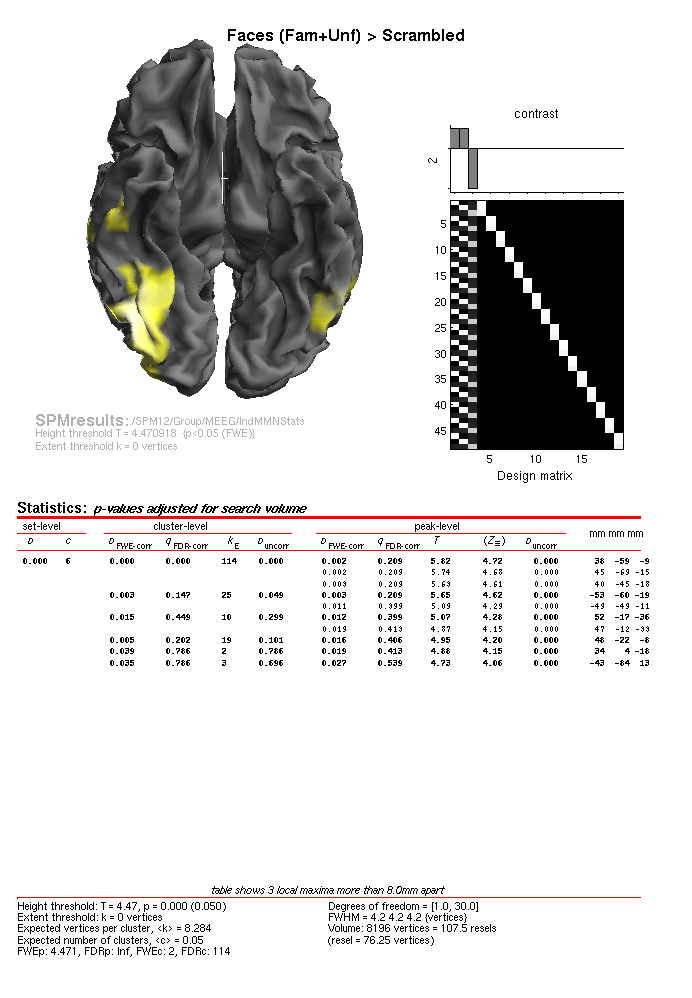
\includegraphics[width=150mm]{multi/figures/figure14}
\caption{\em Group SPM for Faces vs Scrambled power on cortical mesh between 10-20Hz and 100-250ms  across all 16 subjects at \(p<.05\) FWE-corrected, using Individual MNM inversions. \label{multi:fig:14}}
\end{center}
\end{figure}

You can also look at the results of the MSP inversion by selecting the \texttt{SPM.mat} file in the \texttt{MEEG/IndMSPStats} directory. This will not reveal any face-related activations that survive \(p<.05\) FWE-corrected. The likely reason for this is that the sparse solutions for each individual subject are less likely to overlap at the group level (than the ``smoother'' minimum-norm solution). If you change the threshold to \(p<.001\) uncorrected, you will see some activation in posterior right fusiform. However, we can improve the MSP recontructions by pooling across subjects when actually inverting the data -- so-called ``group inversion'' that we consider next.

\section{Group Source Reconstruction}

Because of the indeterminacy of the inverse problem, it is helpful to provide as many constraints as possible. One constraint is to assume that every subject has the same underlying source generators, that are simply seen differently at the sensors owing to different anatomy (head models) and different positions with respect to the sensors (forward models). In the PEB framework, this corresponds to assuming the same set of source priors across subjects (allowing for different sensor-level noise; see [Henson et al, 2011]). This group-based inversion can be implemented in SPM simply by selecting multiple input files to the inversion routine, which can be scripted like this (using the same batch file as before, noting that this includes two inversions -- MNM and MSP -- hence the two inputs of the same data files below):

%\begin{lstlisting}[style=Matlab-editor,basicstyle=\mlttfamily\footnotesize]
%jobfile = {fullfile(scrpth,'batch_localise_evoked_job.m')};
%tmp = cell(nsub,1);
%for s = 1:nsub
%    tmp{s} = spm_select('FPList',fullfile(outpth,subdir{s},'MEEG'),'^apMcbdspmeeg.*\.mat');
%end
%inputs = cell(4,1);
%inputs{1} = cellstr(strvcat(tmp{:}));
%inputs{2} = {''};  % No fMRI priors
%inputs{3} = cellstr(strvcat(tmp{:}));
%inputs{4} = {''};  % No fMRI priors
%spm_jobman('serial', jobfile, '', inputs{:});
%\end{lstlisting}

Note that once you have run this, the previous ``individual'' inversions in the data files will have been overwritten (you could modify the batch to add new inversion indices \texttt{3} and \texttt{4}, so as to compare directly the group inversions with the previous individual inversions, but the files will get very big).

\subsection{Group Statistics on Source Reconstructions}

Now we have a new set of 16\(\times\)3 GIfTI images for the power between 10-20Hz and 100-250ms for each subject for each condition after group-inversion, we can put them into the same repeated-measures ANOVA that we used above, i.e., the \texttt{batch\_stats\_rmANOVA\_job.m} file. This can be scripted as (i.e, simply changing the output directories at the start from, e.g, \texttt{IndMSPStats} to \texttt{GrpMSPStats}).

\begin{lstlisting}[style=Matlab-editor,basicstyle=\mlttfamily\footnotesize]
srcstatsdir{1} = fullfile(outpth,'MEEG','GrpMSPStats');
srcstatsdir{2} = fullfile(outpth,'MEEG','GrpMNMStats');

jobfile = {fullfile(scrpth,'batch_stats_rmANOVA_job.m')};

for val = 1:length(srcstatsdir)
    if ~exist(srcstatsdir{val})
        eval(sprintf('!mkdir %s',srcstatsdir{val}));
    end
    
    inputs  = cell(nsub+1, 1);    
    inputs{1} = {srcstatsdir{val}};    
    for s = 1:nsub
        inputs{s+1,1} = cellstr(strvcat(spm_select('FPList',fullfile(outpth,subdir{s},'MEEG'),sprintf('^apMcbdspmeeg_run_01_sss_%d.*\.gii',val))));   
    end
    
    spm_jobman('serial', jobfile, '', inputs{:});
end
\end{lstlisting}

When it has run, press ``Results'' from the SPM Menu window and select the \texttt{SPM.mat} file in the relevant output directories. You will notice that the results for minimum norm have not changed much -- a lot of voxels remain significant after correction, but in a broadly distributed swathe of ventral temporal lobe. For the results in the \texttt{MEEG/GrpMSPStats} directory, there is a small anterior right temporal cluster that survives correction. But if you lower the threshold to \(p<.001\) uncorrected, you should see results like in Figure~\ref{multi:fig:15}, which includes more focal regions in the ventral temporal lobe, and importantly, more such regions that for the individual MSP inversions the \texttt{MEEG/IndMSPStats} directory (demonstrating the advantage of group-based inversion).

\begin{figure}
\begin{center}
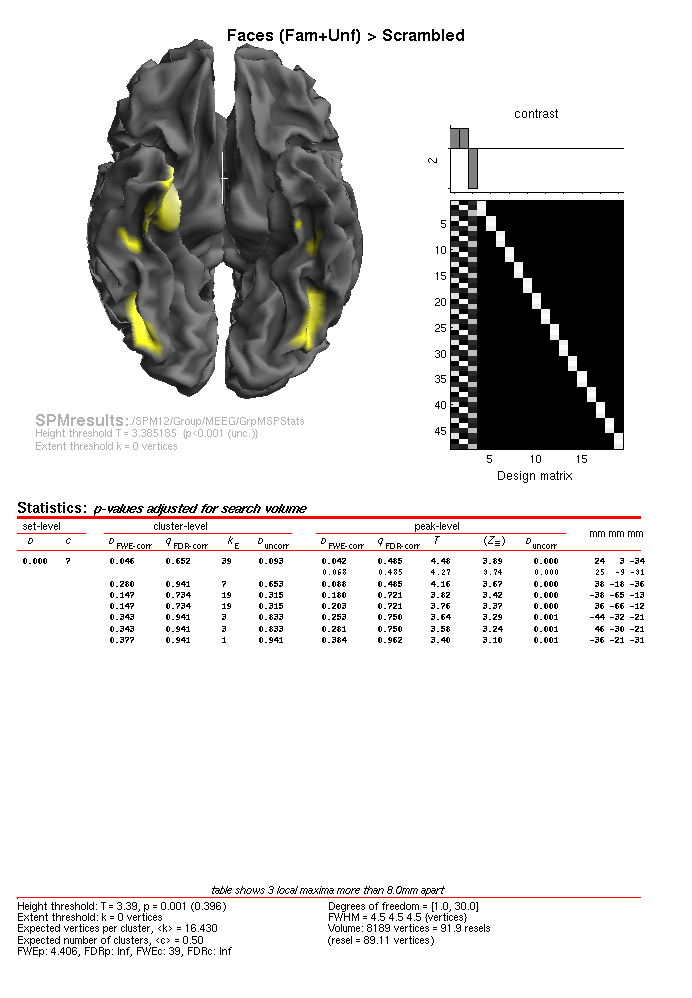
\includegraphics[width=150mm]{multi/figures/figure15}
\caption{\em Group SPM for Faces vs Scrambled power on cortical mesh between 10-20Hz and 100-250ms  across all 16 subjects at \(p<.001\)uncorrected, using Group-optimised MSP. \label{multi:fig:15}}
\end{center}
\end{figure}

\section{Group MEEG Source Reconstruction with fMRI priors}

Finally, in an example of full multi-modal integration, we will use the significant clusters in the group fMRI analysis as separate spatial priors for the group-optimised source reconstruction of the fused MEG and EEG data (see [Henson et al, 2011]). Each cluster becomes a separate prior, allowing for fact that activity in those clusters may occur at different post-stimulus times.

This group-based inversion can be implemented in SPM simply by selecting the binary (thresholded) image we created from the group fMRI statistics (\texttt{fac-scr\_fmri\_05\_cor.nii} in the \texttt{BOLD} directory), which contains non-zero values for voxels to be included in the clustered priors. This is simply an option in the inversion module, so can scripted like this (using the same batch file as before, noting that this includes two inversions -- MNM and MSP -- hence the two inputs of the same data files below):

\begin{lstlisting}[style=Matlab-editor,basicstyle=\mlttfamily\footnotesize]
jobfile = {fullfile(scrpth,'batch_localise_evoked_job.m')};
tmp = cell(nsub,1);
for s = 1:nsub
    tmp{s} = spm_select('FPList',fullfile(outpth,subdir{s},'MEEG'),'^apMcbdspmeeg.*\.mat');
end
inputs = cell(4,1);
inputs{1} = cellstr(strvcat(tmp{:}));
inputs{2} = {fullfile(outpth,'BOLD','fac-scr_fmri_05cor.nii')};  % Group fMRI priors
inputs{3} = cellstr(strvcat(tmp{:}));
inputs{4} = {fullfile(outpth,'BOLD','fac-scr_fmri_05cor.nii')};  % Group fMRI priors
spm_jobman('serial', jobfile, '', inputs{:});
\end{lstlisting}

Note again that once you have run this, the previous ``group'' inversions in the data files will have been overwritten (you could modify the batch to add new inversion indices \texttt{5} and \texttt{6}, so as to compare with previous inversions above, but the file will get very big). Note also that we have used group-defined fMRI priors, but the scripts can easily be modified to define fMRI clusters on each individual subject's 1st-level fMRI models, and use subject-specific source priors here.

\subsection{Group Statistics on Source Reconstructions}

After running the attached script, we will have a new set of 16\(\times\)3 GIfTI images for the power between 10-20Hz and 100-250ms for each subject for each condition after group-inversion using fMRI priors, and can put them into the same repeated-measures ANOVA that we used above, i.e. the \texttt{batch\_stats\_rmANOVA\_job.m} file. This can be scripted as (i.e. simply changing the output directories at the start from, e.g. \texttt{GrpMNMStats} to \texttt{fMRIGrpMNMStats}).

\begin{lstlisting}[style=Matlab-editor,basicstyle=\mlttfamily\footnotesize]
srcstatsdir{1} = fullfile(outpth,'MEEG','fMRIGrpMSPStats');
srcstatsdir{2} = fullfile(outpth,'MEEG','fMRIGrpMNMStats');

jobfile = {fullfile(scrpth,'batch_stats_rmANOVA_job.m')};

for val = 1:length(srcstatsdir)
    if ~exist(srcstatsdir{val})
        eval(sprintf('!mkdir %s',srcstatsdir{val}));
    end
    
    inputs  = cell(nsub+1, 1);    
    inputs{1} = {srcstatsdir{val}};    
    for s = 1:nsub
        inputs{s+1,1} = cellstr(strvcat(spm_select('FPList',fullfile(outpth,subdir{s},'MEEG'),...
            sprintf('^apMcbdspmeeg_run_01_sss_%d.*\.gii$',val))));   
    end
    
    spm_jobman('serial', jobfile, '', inputs{:});
end
\end{lstlisting}

When it has run, press ``Results'' from the SPM Menu window an select the \texttt{SPM.mat} file from the \texttt{fMRIGrpMSPStats} directory, and choose an uncorrected threshold of \(p<.001\). You should see results like in Figure~\ref{multi:fig:16}, which you can compare to Figure~\ref{multi:fig:15}. The fMRI priors have improved consistency across subjects, even in medial temporal lobe regions, as well as increasing significance of more posterior and lateral temporal regions (cf., Figure~\ref{multi:fig:11}, at \(p<.001\) uncorrected).

\begin{figure}
\begin{center}
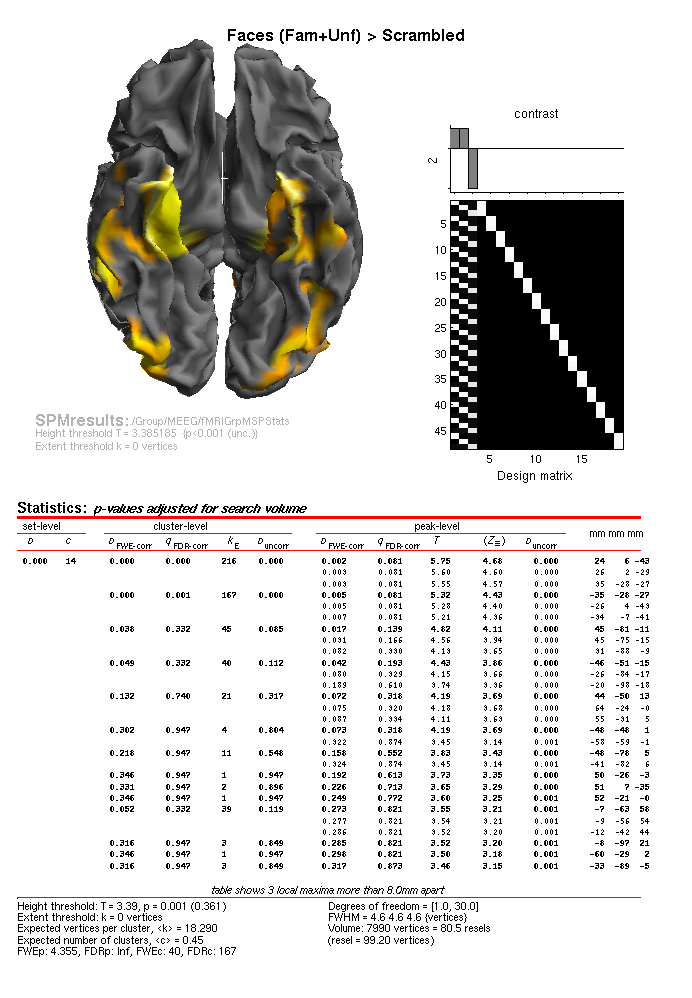
\includegraphics[width=150mm]{multi/figures/figure16}
\caption{\em Group SPM for Faces vs Scrambled power on cortical mesh between 10-20Hz and 100-250ms  across all 16 subjects at \(p<.001\) uncorrected, using Group-optimised MSP and fMRI priors. \label{multi:fig:16}}
\end{center}
\end{figure}

\section{References}

\noindent 1. Henson, R.N., Mattout, J., Phillips, C. and Friston, K.J. (2009). Selecting forward models for MEG source-reconstruction using model-evidence. Neuroimage, 46, 168-176. \\
\noindent 2. Henson, R.N., Wakeman, D.G., Litvak, V. and Friston, K.J. (2011). A Parametric Empirical Bayesian framework for the EEG/MEG inverse problem: generative models for multisubject and multimodal integration. Frontiers in Human Neuroscience, 5, 76, 1-16. \\
\noindent 3. Wakeman, D.G. and Henson, R.N. A multi-subject, multi-modal human neuroimaging dataset. Scientific Data, 2:150001. \\

\section{Acknowledgements}
This work was supported by MRC (A060\_MC\_5PR10). The author (RNH) thanks Rebecca Beresford, Hunar Abdulraham, Daniel Wakeman, Guillaume Flandin and Vladimir Litvak for their help.
